\documentclass[12pt, letterpaper]{article}

\usepackage[T1]{fontenc}
\usepackage[utf8]{inputenc}
\usepackage[frenchb]{babel}
\usepackage{gensymb}
\usepackage{latexsym}
\usepackage{titlesec}
\usepackage{marvosym}
\usepackage{enumitem}
\usepackage[pdftex, hidelinks]{hyperref}
\usepackage{graphicx}
\usepackage{rotating}
\usepackage{caption}

\frenchbsetup{StandardItemLabels=true}

\author{Edorh François (EDOF19059507), Guison Vianney (GUIV30069402)}
\title{Rapport TP1 de Métaheuristique en Optimisation}


\begin{document}
\maketitle
\tableofcontents
\newpage

\section{Méthodes implémentées}
L'algorithme génétique est utilisable sur toute fonction à $n$
arguments, avec $n >= 1$.

\subsection{Crossovers}

Toutes les méthodes de crossover sont dans le fichier Crossover.m.\\
Elles sont stockées dans la variable globale CROSSOVER.

\subsubsection{Encodage binaire}
Les variables réelles sont converties en entier entre 0 et $2^l-1$,
avec $l$ la longueur du chromosome ($1 <= l <= 53$).
\\
Chaque variable est représentée par un chromosome différent, chaque
chromosome a la même longueur.
\\
\\
Les méthodes de crossover en encodage binaire suivantes ont été
implémentées:
\begin{itemize}
\item single-point crossover,
  
\item multi-point crossover, avec un paramètre de contrôle $n$ compris
entre 1 et $l - 1$,
  
\item uniform crossover, avec deux variantes:
  \begin{itemize}
  \item un paramètre $p$ représentant une probabilité constante,
    
  \item deux paramètres de contrôle $p$ et $t$, où la probabilité
    d'une paire $(a, b)$ est donnée par $P(T(a), T(b))$.
    
  \end{itemize}
\end{itemize}

\subsubsection{Encodage réel}

Les méthodes de crossover sur valeurs réelles suivantes ont été
implémentés:

\begin{itemize}
\item whole arithmetic crossover,
  
\item local arithmetic crossover,
  
\item blend crossover (ou $BLX-\alpha$), avec un paramètre de contrôle
  $\alpha$ (valeur par défaut de 0.5),
  
\item simulated binary crossover, avec un paramètre de contrôle $n >= 0$.
\end{itemize}


\subsubsection{Au choix}

La méthode de crossover choisie est \textit{1-Bit Adaptation}. C'est une
méthode de crossover en encodage binaire.\\
\\
Le principe est de définir deux méthodes de crossover différentes que
l'on associe à la valeur 1 ou 0. Lors du crossover, on regarde le
dernier bit des parents.\\
Si ils sont égaux, la méthode de crossover utilisée est celle associée
à la valeur de ce bit (1 ou 0).
\\
Si ils sont différents, un nombre aléatoire $u$ entre 0 et 1 indique
quelle méthode utiliser: si $u < 0.5$, on utilise la méthode associée
à 0, sinon on utilise celle associée à 1.
\\
\\
Ajout personnel: étant donné que chaque variable possède un
chromosome, avant la vérification du dernier bit des parents, un
$\oplus$ (xor) entre les variables d'un même parent est
effectué. C'est le résultat de ce calcul qui est comparé avec celui de
l'autre parent.
\\
$\oplus$ a été choisie car c'est la seule fonction binaire à deux
opérandes qui produit 0 et 1 dans les mêmes proportions.

\subsection{Mutations}

Toutes les méthodes de mutation sont dans le fichier Mutation.m.\\
Elles sont stockées dans la variable globale MUTATION.

\subsubsection{Encodage binaire}

La méthode de mutation binaire implémentée est la mutation bit-flip.

\subsubsection{Encodage réel}

Les méthodes de mutation sur valeurs réelles suivantes ont été implémentées:

\begin{itemize}
\item uniform mutation,
  
\item boundary mutation,
  
\item normal mutation, avec un paramètre $\sigma$ (nombre ou tableau),
  
\item polynomial mutation, avec un paramètre de contrôle $n >= 0$,
  
\item non-uniform mutation, avec un paramètre de contrôle $b$.
\end{itemize}

\subsection{Sélections}

Toutes les méthodes de sélection sont dans le fichier Sélection.m.\\
Elles sont stockées dans la variable globale SELECTION.
\\
\\
Les méthodes de sélection suivantes ont été implémentées:

\begin{itemize}
  
\item wheel selection,
	
\item stochastic universal sampling,
	
\item tournament selection, avec un paramètre de contrôle $k$, compris
  entre 1 et $N$, le nombre d'individus,
	
\item unbiased tournament selection, avec un paramètre de contrôle $k$,
  compris entre 1 et $N$, le nombre d'individus,
	
\item truncation selection, avec un paramètre $c$ compris entre 1 et $N$,
  le nombre d'individus, où $N/c$ correspond au nombre d'individus
  utilisés dans la sélection.
\end{itemize}

\subsection{Faisabilité}

Les deux méthodes permettant d'assurer la faisabilité d'une solution
ont été implémentées dans Clamp.m.\\
Elles sont stockées dans la variable globale CLAMP.

\subsection{Changement de fitness}

Toutes les méthodes de changement de fitness sont dans le fichier
\\\-FitnessChange.m.\\
Elles sont stockées dans la variable globale FITNESS\_CHANGE.
\\\\
Les méthodes de changment de fitness suivantes ont été implémentées:
\begin{itemize}
\item échelle linéaire,
  
\item troncature sigma, avec un paramètre de contrôle $c$ dans $[1, 5]$.
\end{itemize}
Dans le cas d'une maximisation où des fitness négatives sont produites,
l'ensemble des fitness est translatée de sorte à ce que la fitness
minimale soit 0.\\
Cela revient à maximiser: $f'(x) = f(x) - min(f(x))$.
\\
\\
Dans le cas d'une minimisation, la méthode du transfert de fitness est
utilisée.\\
C'est à dire que minimiser $f(x)$ revient à maximiser
$f'(x) = max(f(x)) - f(x)$.

\subsection{Classement}
Toutes les méthodes de classement sont dans le fichier Ranking.m.\\
Elles sont stockées dans la variable globale RANKING.
\\\\
Les méthodes de classement suivantes ont été implémentées:
\begin{itemize}
\item linéaire, avec un paramètre de contrôle $\alpha$ ($\beta$ est déduit),
  
\item linéaire (2ème méthode), avec un paramètre de contrôle $t$ dans $[0, 1]$ (pour calculer $r$; $q$ est déduit),
  
\item non-linéaire, avec un paramètre de contrôle $\alpha$ dans $]0, 1[$.
\end{itemize}

\subsection{Stratégie \textit{Steady State}}

Un paramètre $\lambda$ permet d'utiliser la stratégie \textit{steady state}
($\lambda = 1$ ou $2$) ou non ($\lambda = -1$).

\subsection{Critères d'arrêt}

Toutes les méthodes d'arrêt sont dans le fichier StopCriteria.m.\\
Elles sont stockées dans la variable globale STOP\_CRITERIA.
\\\\
Les critères d'arrêt suivants ont été implémentés:
\begin{itemize}
\item time,
  
\item threshold, avec deux paramètres de contrôle:
  \begin{itemize}
  \item $r$, la relation entre la fitness et la limite $t$ ($>=$, $<=$,
    ...),
    
  \item $t$, la limite fixée.
  \end{itemize}
	
\item variance, avec un paramètre de contrôle $v$: l'algorithme
  s'arrête quand la variance de la fitness est inférieur ou égale à
  $v$,
	
\item min-max ratio, avec un paramètre de contrôle $r$, l'algorithme
  s'arrête lorsque le rapport entre la valeur maximale de la fitness
  et sa valeur minimale est proche de $r$,
	
\item mean-change rate, avec un paramètre de contrôle $cr$:
  l'algorithme s'arrête quand la différence entre la valeur moyenne de
  la fitness actuelle et la précédente est inférieur ou égale à $cr$,
\end{itemize}

N.B: Même si un critère d'arrêt différent du temps est défini,
l'algorithme ne dépassera pas le nombre d'itérations maximum donné.

\section{Benchmarks}

\subsection{Configuration}
Dans les deux problèmes d'optimisation, nous utilisons la fonction
donnée comme fonction de fitness.
\\
Le maximum de la fonction de Rosenbrock négative est en
$(1.733..., 3)$. La valeur associée est 2.0025.

Nous avons choisi un critère d'arrêt $f(x, y) > 2.002$.

Le minimum de la fonction de Griewank est en $(0, 0)$. La valeur associée est
0.

Nous avons choisi un critère d'arrêt $f(x, y) < 10^{-4}$.
\\
\\
$G_{max}$ est fixé à 250.
\\
\\
En encodage réel, nous utilisons \textit{boundary mutation} comme fonction
de mutation.
\\
Lorsque qu'une solution dépasse l'interval, nous lui assignons ses
valeurs extrêmes (\textit{default clamp}).
\\
\\
Les autres paramètres sont les paramètres par défaut de l'algorithme.
\\
Chaque combinaison a été effectuée 50 fois.

\subsection{Affichage}
Pour chaque test, deux affichages sont produits:
\begin{itemize}
  
\item le logarithme (en base 10) du nombre d'itérations avant que
  l'algorithme ne s'arrête,
  
\item le logarithme (en base 10) de l'erreur entre la meilleur valeur
  trouvée et le maximum possible de la fonction de fitness. L'erreur
  attendue (par rapport au critère d'arrêt) est représentée par la
  ligne verte. Les valeurs au dessus de cette ligne ne satisfont pas
  le critère d'arrêt.

\end{itemize}

\subsection{Encodage réel}

(Voir Figures \ref{fig:r_blx_ut_08_001} - \ref{fig:r_blx_sus}
et \ref{fig:g_blx_ut_08_001} - \ref{fig:g_blx_sus})
\\
\\
Nous avons fait varier les paramètres suivants:
\begin{itemize}
\item $N$, le nombre d'individus: 100, 200, 500 et 1000,
\item $\alpha$, le paramètre de contrôle de la fonction de crossover \textit{BLX-$\alpha$}: 0.25, 0.5 et 0.75,
\item $k$, le paramètre de contrôle de la fonction de sélection par tournoi: 2 et 5,
\item $P_C$, la probabilité de crossover: 0.8 et 0.65,
\item $P_M$, la probabilité de mutation: 0.001 et 0.01.
\end{itemize}

Nous avons ensuite comparé différentes fonctions de sélection (\textit{wheel
selection} et \textit{stochastic universal sampling}).

\subsubsection{Commun}

On remarque que le nombre d'individus influe grandement sur le nombre
d'itérations nécessaire pour satisfaire le critère d'arrêt: plus il
est grand, plus l'algorithme est performant.
\\
Plus $k$ est grand, meilleur est l'algorithme.

\subsubsection{Rosenbrock}
On peut remarquer que pour une combinaison donnée, plus le paramètre
$\alpha$ est grand, meilleur est l'algorithme.
\\
Une probabilité de crossover modérée ($P_C = 0.65$) ainsi qu'une
faible probabilité de mutation ($P_M = 0.01$) semble être préférables.
\\
La méthode du tournoi avec $k = 5$ semble la meilleure fonction de
sélection suivie de \textit{wheel selection}, la sélection par tournoi
avec $k = 2$ et finalement \textit{stochastic universal sampling}.

\subsubsection{Griewank}
On peut remarquer que pour une combinaison donnée, plus le paramètre
$\alpha$ est petit, meilleur est l'algorithme.
\\
Une grande probabilité de crossover ($P_C = 0.8$) ainsi qu'une très
faible probabilité de mutation ($P_M = 0.001$) semble être
préférables.
\\
La méthode du tournoi est la meilleure fonction de sélection suivie de
\textit{stochastic universal sampling} et de \textit{wheel selection}.

\subsection{Encodage binaire}

(Voir Figures \ref{fig:r_mp_ut} - \ref{fig:r_1b_ut}
et \ref{fig:g_mp_ut} - \ref{fig:g_1b_ut})

Nous avons comparé les performances de \textit{multi-point crossover} (avec
$n$: 1, 2 et 10) par rapport à \textit{1-bit adaptation crossover} paramétré
avec les fonctions de crossover suivantes:
\begin{itemize}
\item \textit{multi-point crossover}, avec un paramètre $n$: 1 (\textit{single-point crossover}), 2 (\textit{two-point crossover}),
  
\item \textit{uniform crossover}, avec un paramètre $\alpha$: 0.25, 0.5 et 0.75.
  
\end{itemize}

\subsubsection{Commun}
L'encodage binaire donne des résultats comparables à l'encodage réel.
1-BX semble être plus performant que \textit{multi-point crossover}.

\subsubsection{Rosenbrock}
Les résultats de 1-BX sont parmis les meilleurs lorsque $N = 1000$ et
ce de manière constante (même comparé aux méthodes en encodage réel
précédentes).

\subsubsection{Griewank}
En utilisant \textit{multi-point crossover}, un trop grand nombre $n$
de points semble faire baisser les performances de l'algorithme.

\section{Remarques générales}
Il vaut mieux préférer l'encodage réel à l'encodage binaire si l'on
privilégie le temps de calcul.
\\
\\
\textit{Multi-point crossover} est la fonction de crossover la plus
lente et son temps d'exécution dépend du nombre de points $n$.
\\
\\
Les sélections par tournoi sont plus intéressantes que les autres
sélections au niveau temporel:
\begin{itemize}
\item avec la sélection par tournoi non-biaisée et $k = 2$, il faut
  $0.5s$ pour effectuer 1000 itérations avec 1000 individus,
  
\item avec \textit{wheel selection}, il faut $1.5s$.\\
\end{itemize}

L'utilisation de l'algorithme \textit{steady state} avec un remplacement
par valeur permet de garantir que le meilleur individu de l'itération
$i$ est égal ou meilleur que celui de l'itération $i - 1$.
\\
Cependant, étant donné que la population ne change que très peu à
chaque itération, il est assez rare de trouver un solution acceptable
en peu d'itérations.\\
Par contre, il fonctionne très bien avec une très faible population.
(Voir Figure \ref{fig:r_ss})
\\
Il semble aussi mieux fonctionner en utilisant un système de
classement, bien qu'il faille tout de même compter en milliers
d'itérations (ce qui correspond à $\simeq 0.25s$ par millier).
\\
Le problème de Griewank semble moins adapté à son utilisation.
\\
(Voir Figures \ref{fig:r_ss_test} et \ref{fig:g_ss_test})
\\
\\
\\
On peut trouver une solution au problème de Rosenbrock en une dizaine
d'itérations (et même moins) avec:
\begin{itemize}
\item  $N = 100$,
\item \textit{unbiased tournament} avec un $k >= 4$,
\item \textit{blend crossover} avec $\alpha$ proche ou égale à 1,
\item \textit{boundary mutation}.
\end{itemize}
Cela prend $\simeq 10ms$.\\
(Voir Figure \ref{fig:r_quick})
\\
\\
On peut trouver une solution au problème de Griewank en une vingtaine d'itérations (et même moins) avec:
\begin{itemize}
\item  $N = 500$,
\item \textit{unbiased tournament} avec un $k = 2$,
\item \textit{blend crossover} avec  $\alpha$ proche ou égale à 0,
\item \textit{non-uniform mutation} avec $b = 2$.
\end{itemize}
Cela prend $\simeq 15ms$.\\
(Voir Figure \ref{fig:g_quick})


\newpage

\section{Figures}
\clearpage{}

%% Rosenbrock
\begin{figure}
  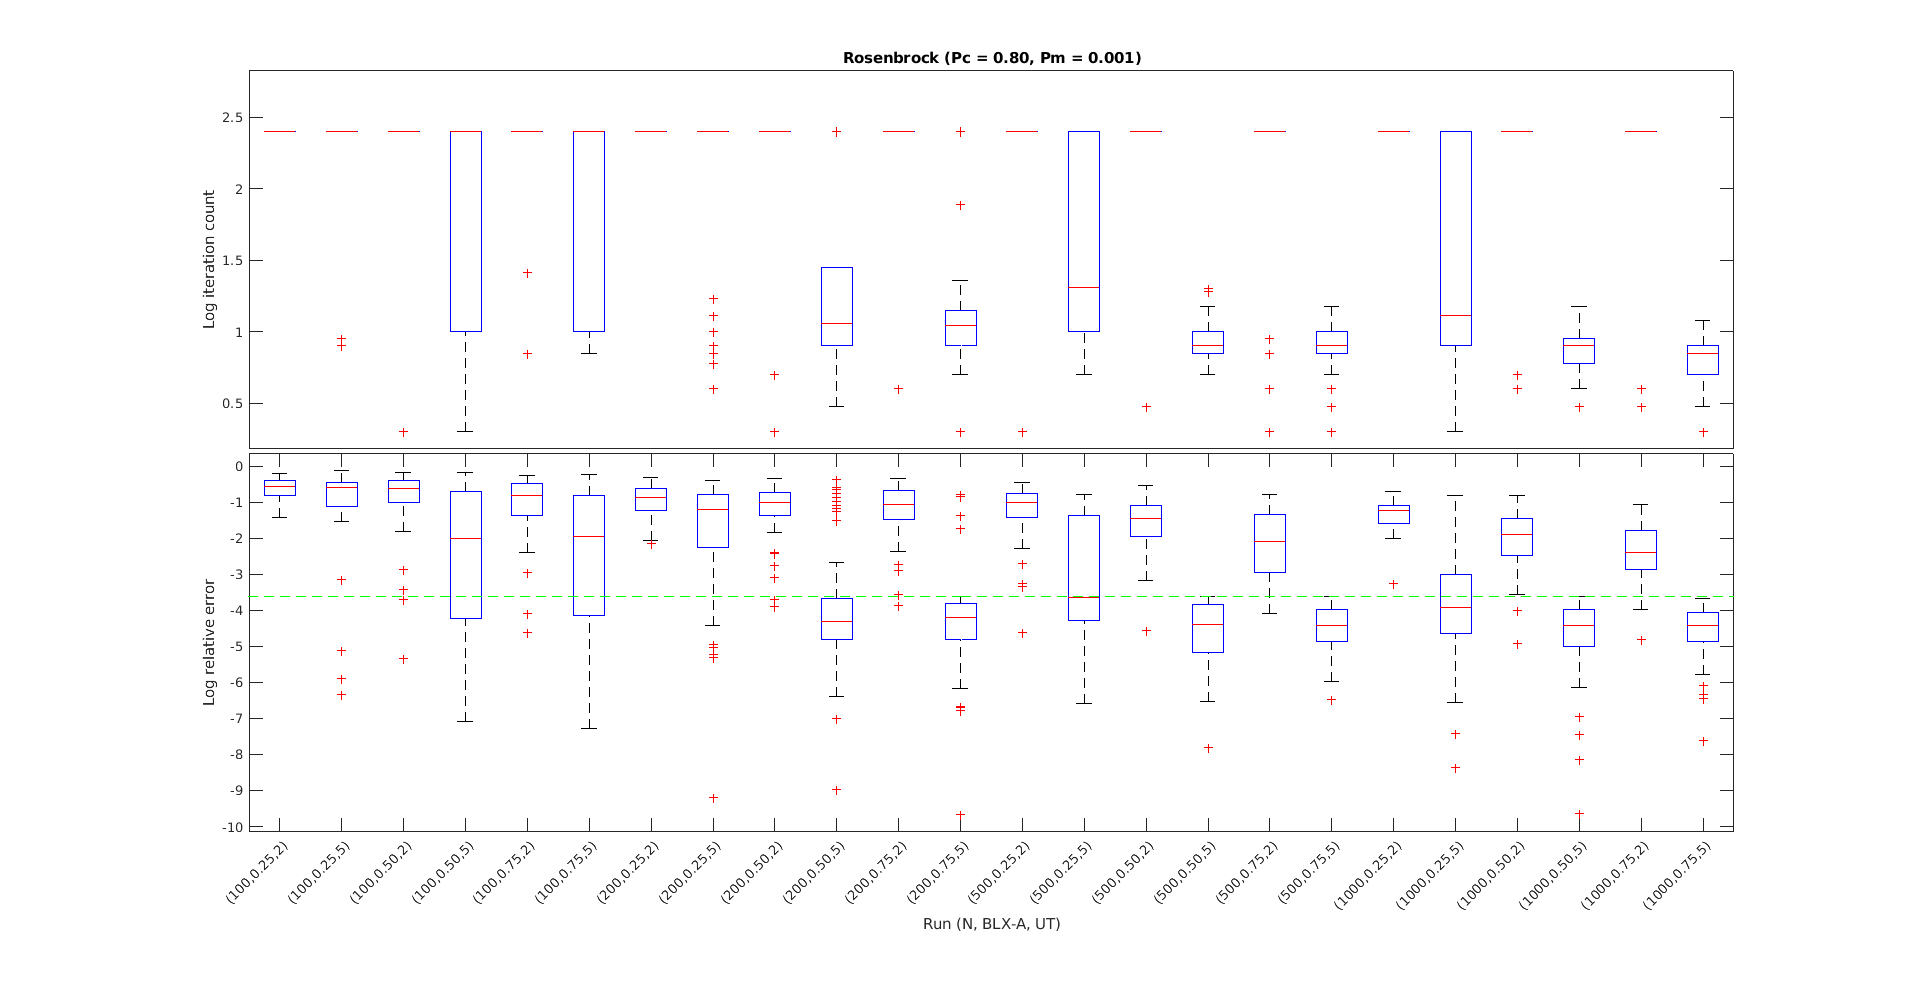
\includegraphics[width=\linewidth]{img/r_blx_ut_08_001.png}
  \centering
  \captionsetup{justification=centering}
  \caption{Rosenbrock - BLX-$\alpha$, Unbiased tournament, $P_C = 0.8$, $P_M = 0.001$}
  \label{fig:r_blx_ut_08_001}
\end{figure}

\begin{figure}
  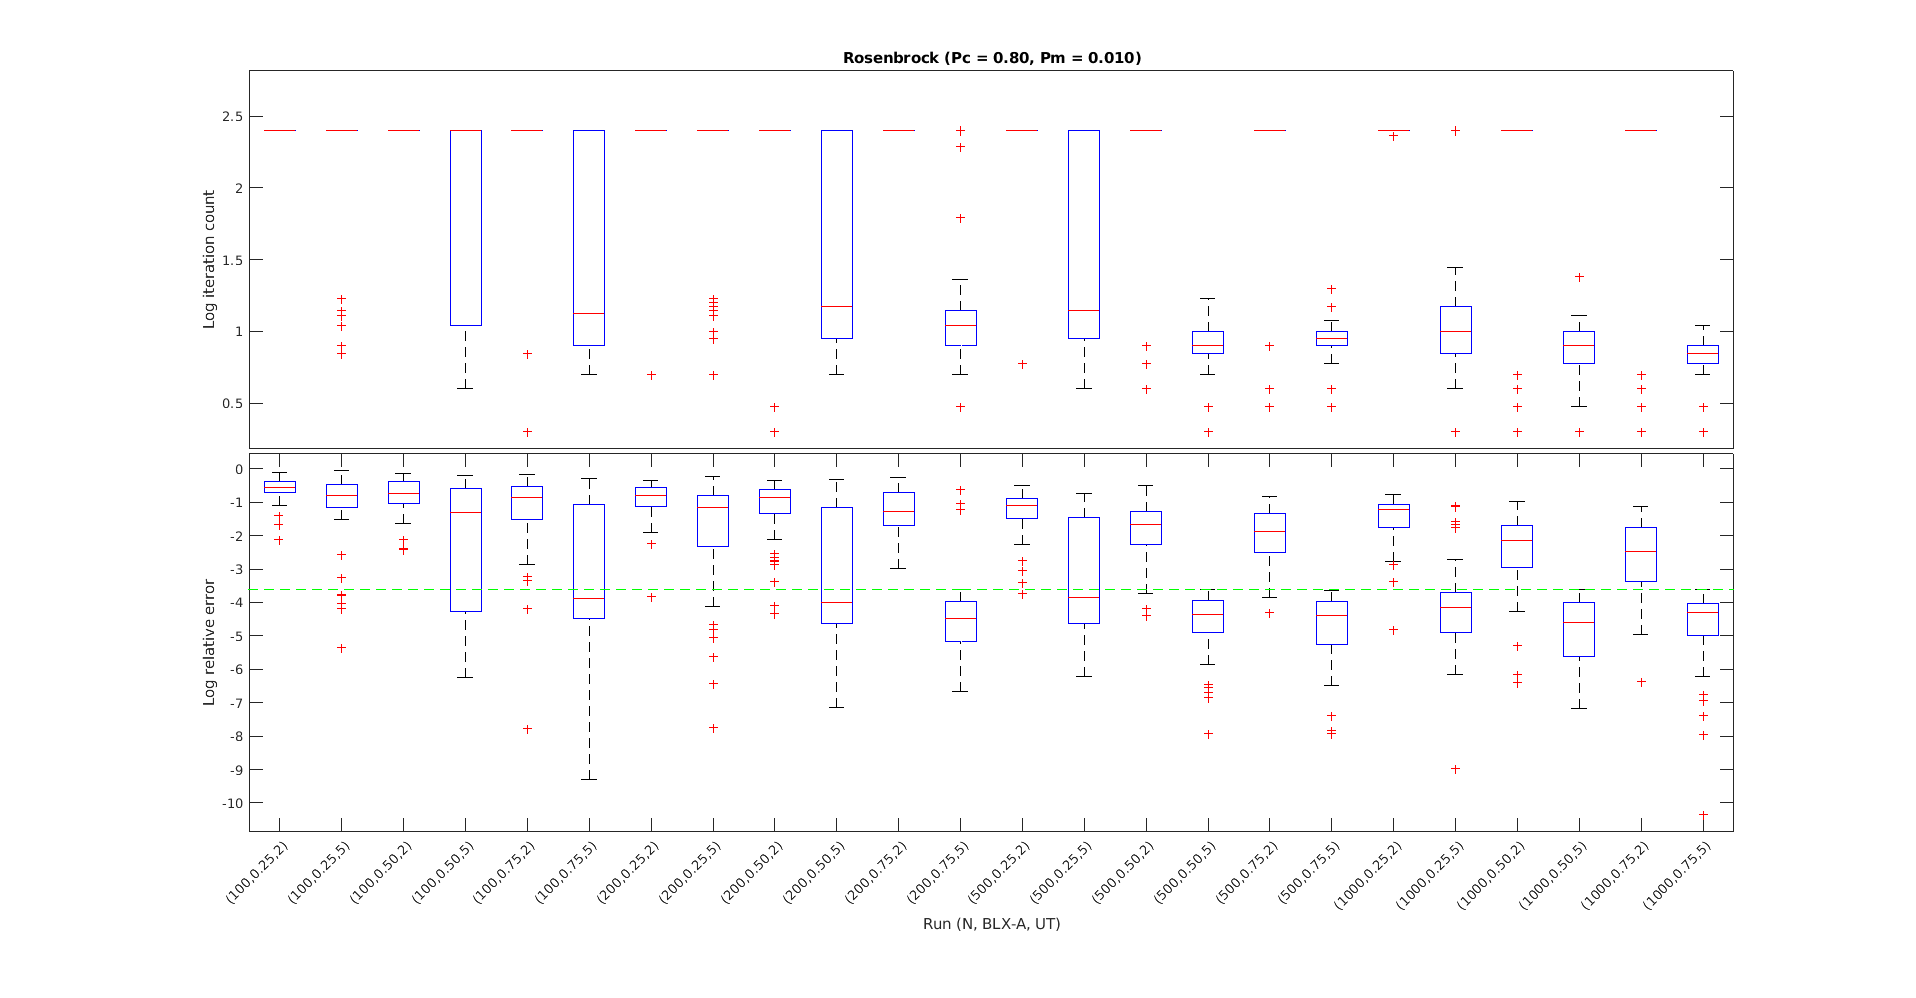
\includegraphics[width=\linewidth]{img/r_blx_ut_08_010.png}
  \centering
  \captionsetup{justification=centering}
  \caption{Rosenbrock - BLX-$\alpha$, Unbiased tournament, $P_C = 0.8$, $P_M = 0.01$}
  \label{fig:r_blx_ut_08_010}
\end{figure}

\begin{figure}
  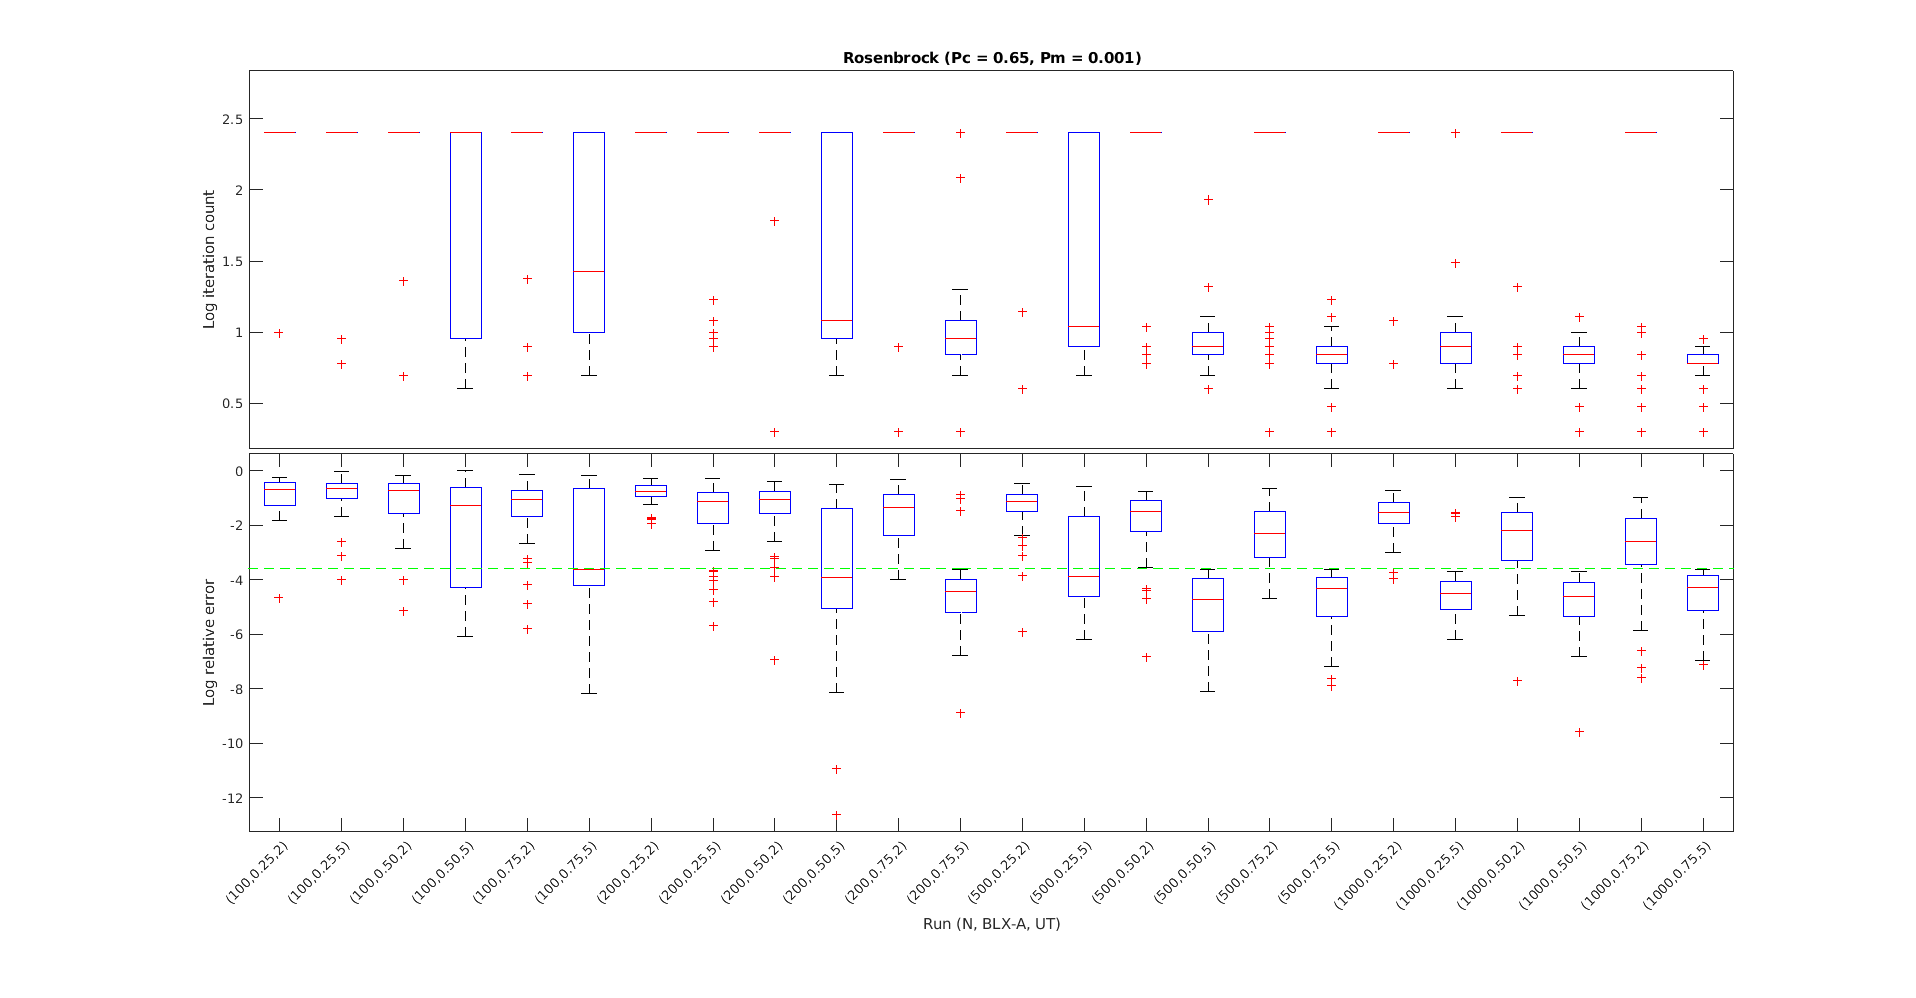
\includegraphics[width=\linewidth]{img/r_blx_ut_065_001.png}
  \centering
  \captionsetup{justification=centering}
  \caption{Rosenbrock - BLX-$\alpha$, Unbiased tournament, $P_C = 0.65$, $P_M = 0.001$}
  \label{fig:r_blx_ut_065_001}
\end{figure}

\begin{figure}
  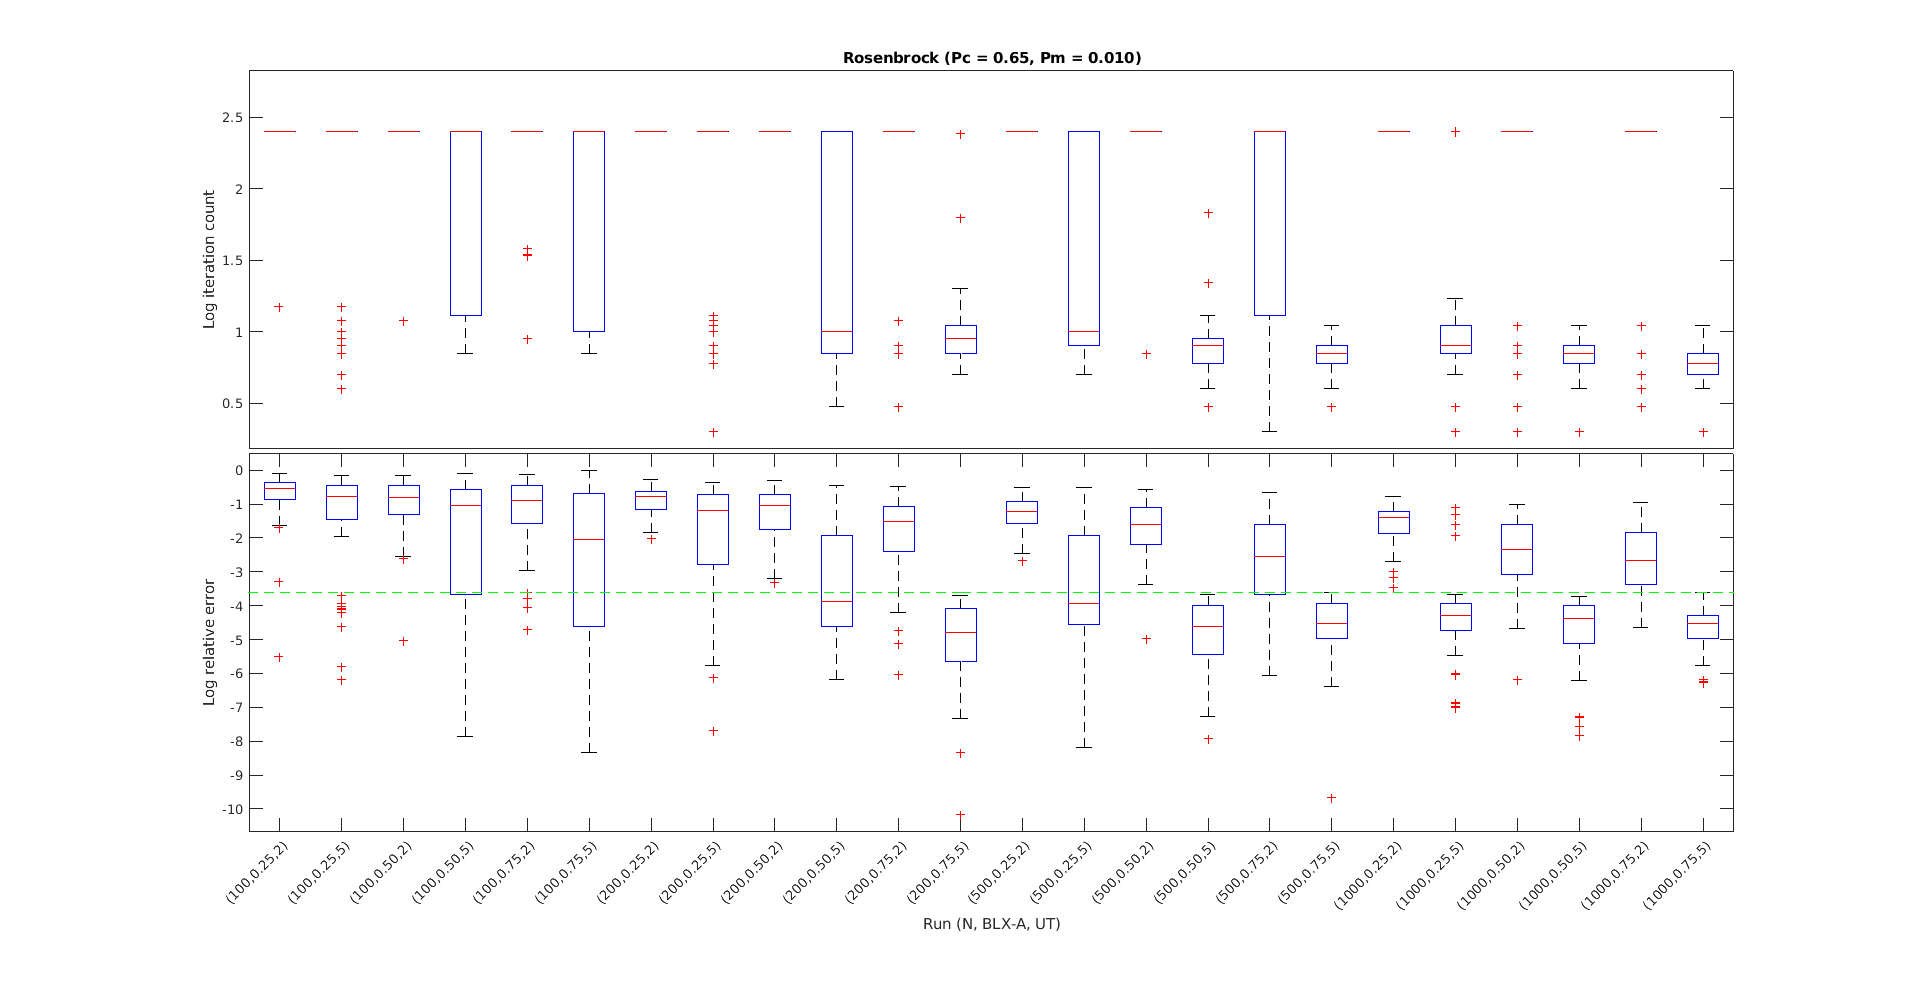
\includegraphics[width=\linewidth]{img/r_blx_ut_065_010.png}
  \centering
  \captionsetup{justification=centering}
  \caption{Rosenbrock - BLX-$\alpha$, Unbiased tournament, $P_C = 0.65$, $P_M = 0.01$}
  \label{fig:r_blx_ut_065_010}
\end{figure}

\begin{figure}
  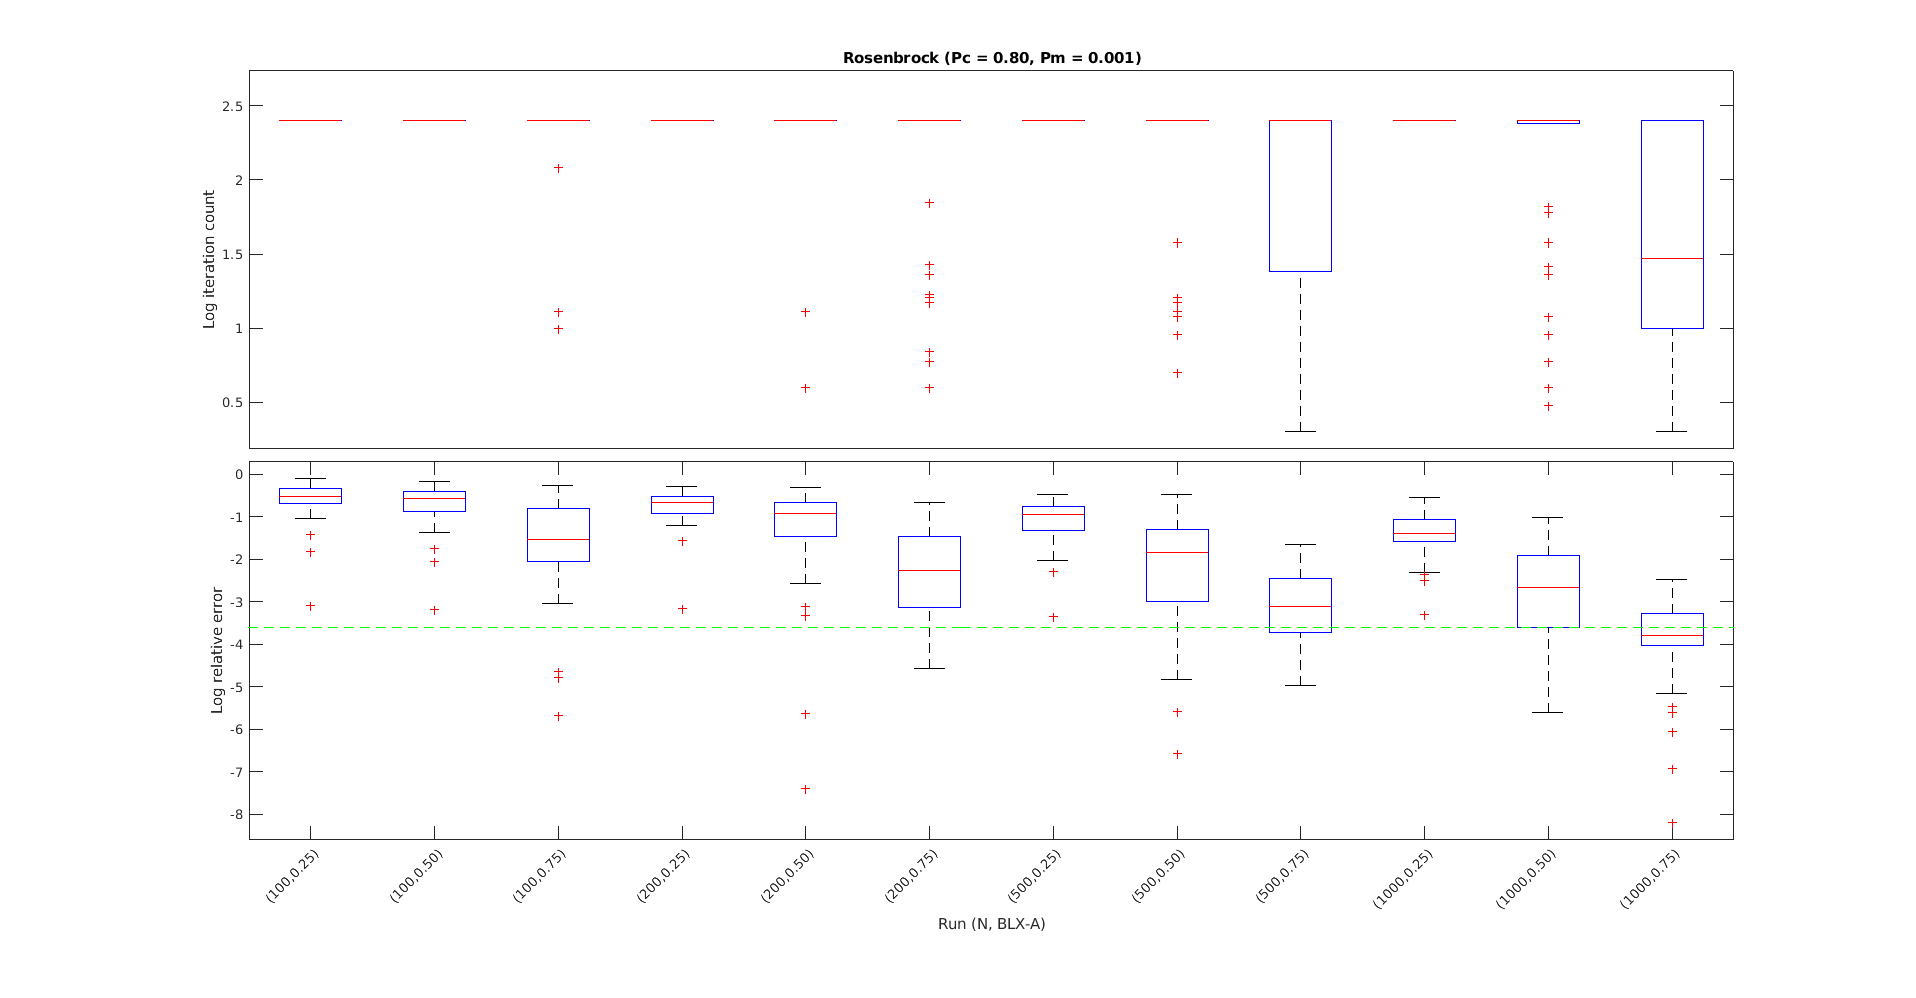
\includegraphics[width=\linewidth]{img/r_blx_w.png}
  \centering
  \captionsetup{justification=centering}
  \caption{Rosenbrock - BLX-$\alpha$, Wheel}
  \label{fig:r_blx_w}
\end{figure}

\begin{figure}
  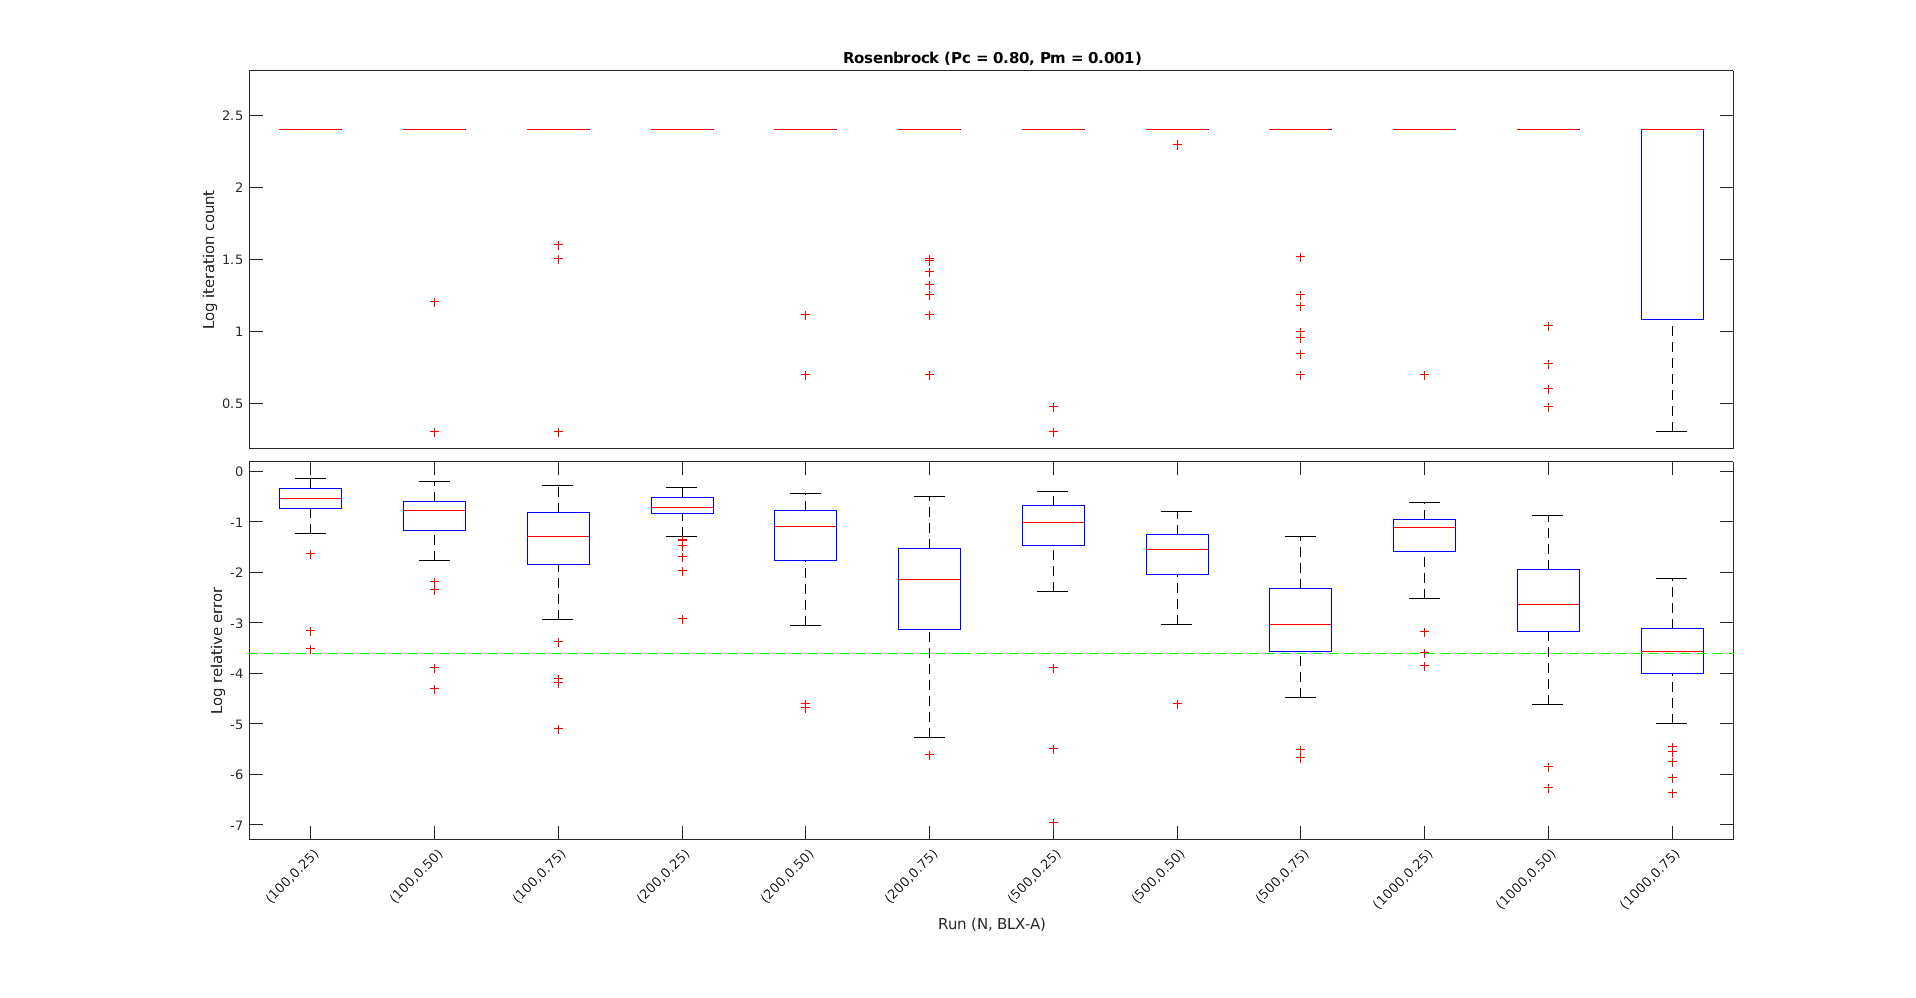
\includegraphics[width=\linewidth]{img/r_blx_sus.png}
  \centering
  \captionsetup{justification=centering}
  \caption{Rosenbrock - BLX-$\alpha$, Stochastic Universal Sampling}
  \label{fig:r_blx_sus}
\end{figure}

\begin{figure}
  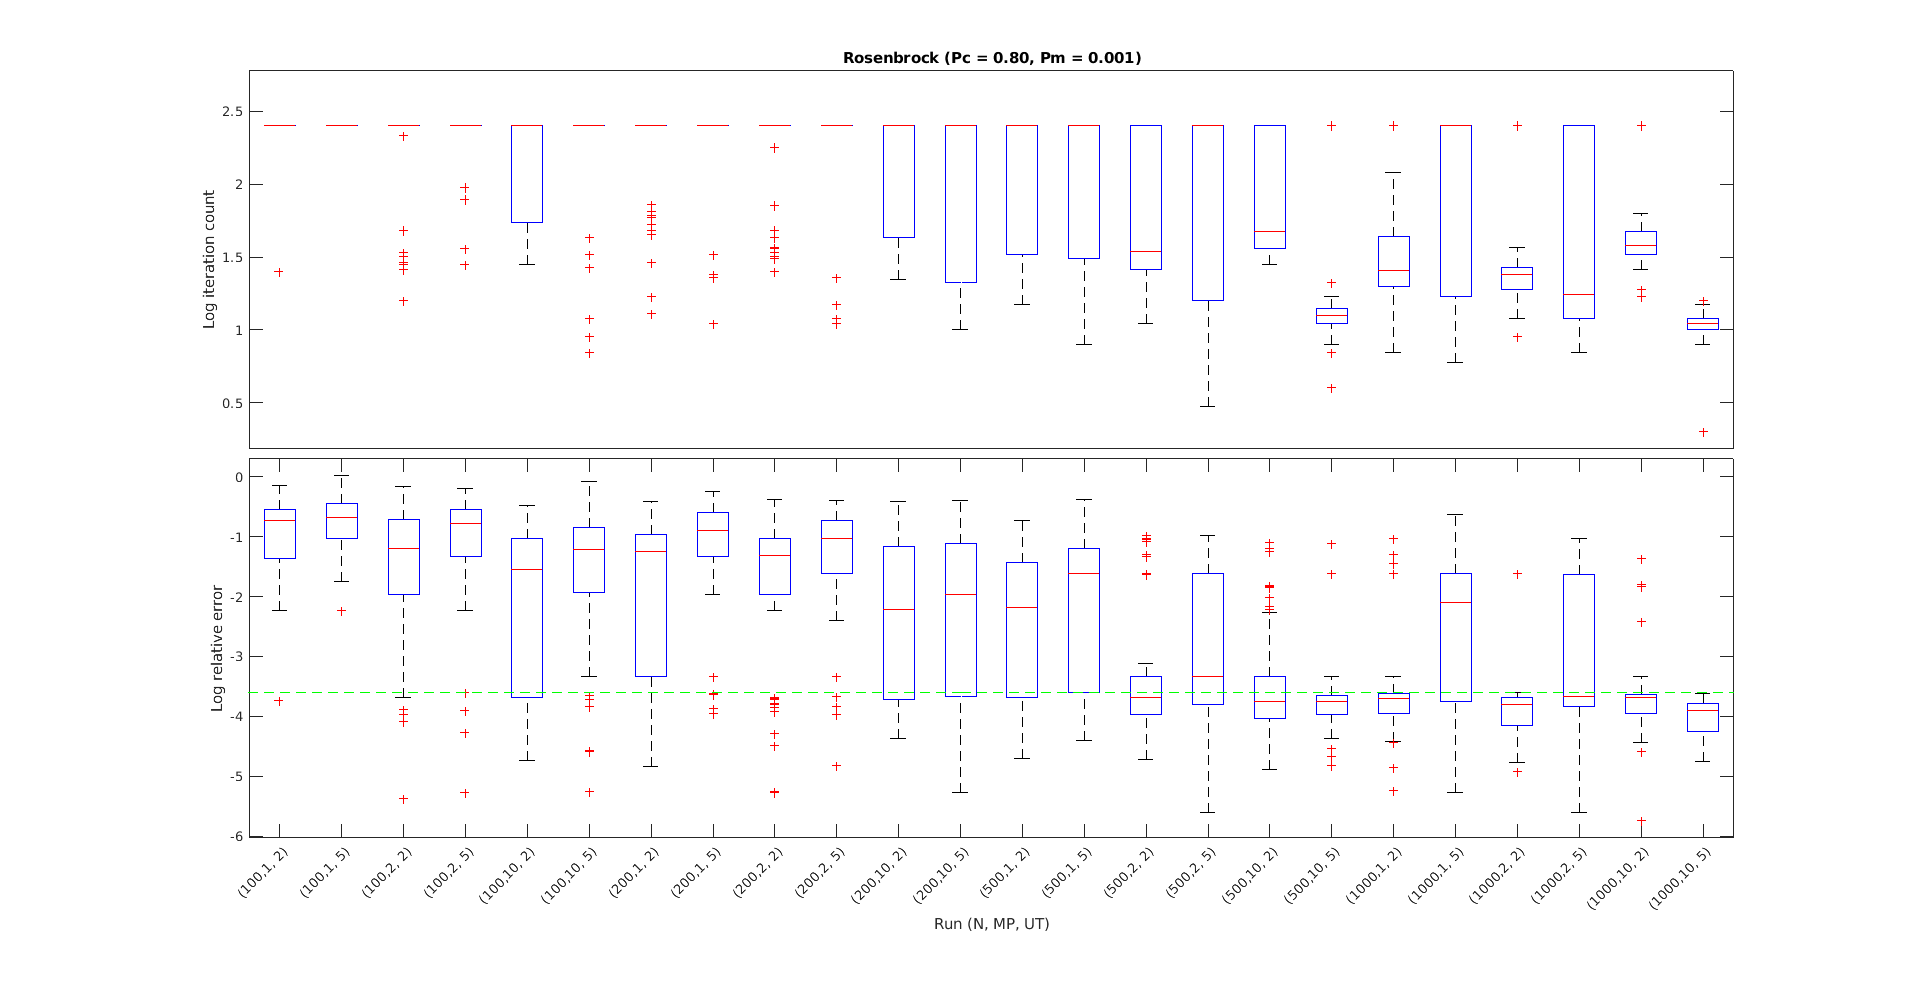
\includegraphics[width=\linewidth]{img/r_mp_ut.png}
  \centering
  \captionsetup{justification=centering}
  \caption{Rosenbrock - Multi-point, Unbiased tournament}
  \label{fig:r_mp_ut}
\end{figure}

\begin{figure}
  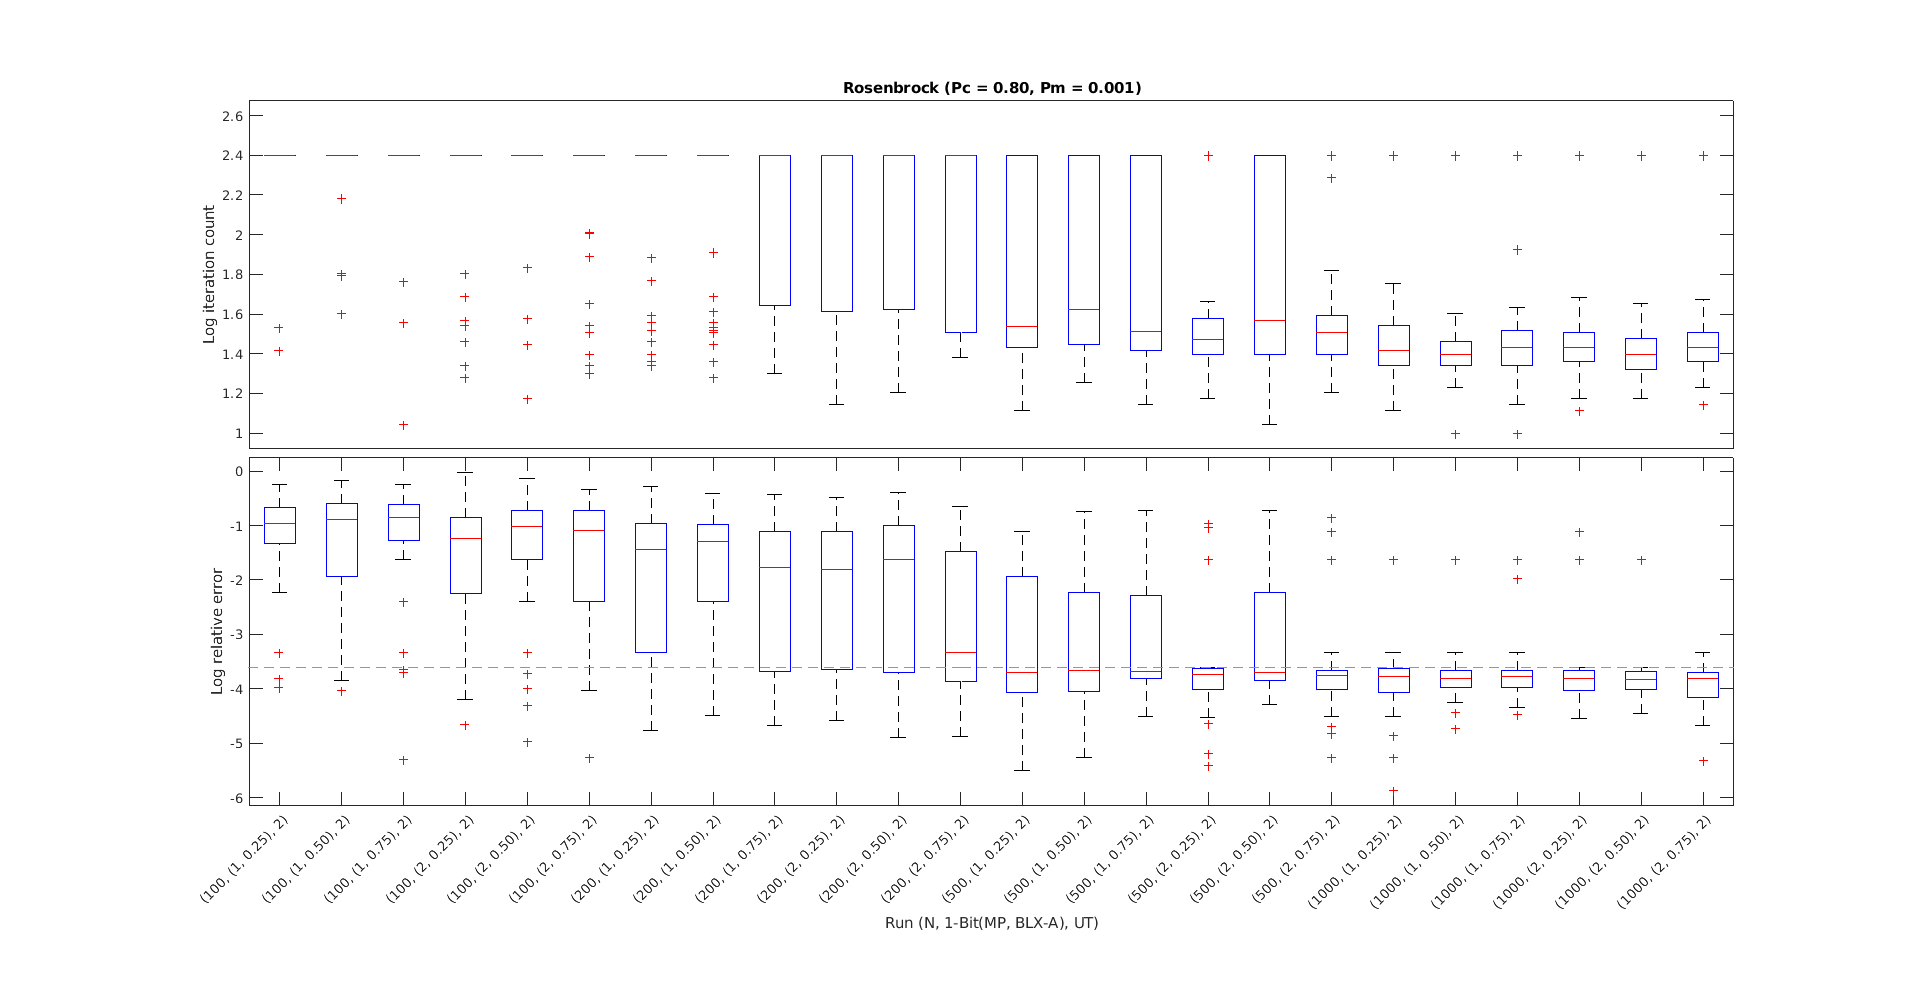
\includegraphics[width=\linewidth]{img/r_1b_ut.png}
  \centering
  \captionsetup{justification=centering}
  \caption{Rosenbrock - 1-Bit Adaptation, Unbiased tournament}
  \label{fig:r_1b_ut}
\end{figure}

\begin{figure}
  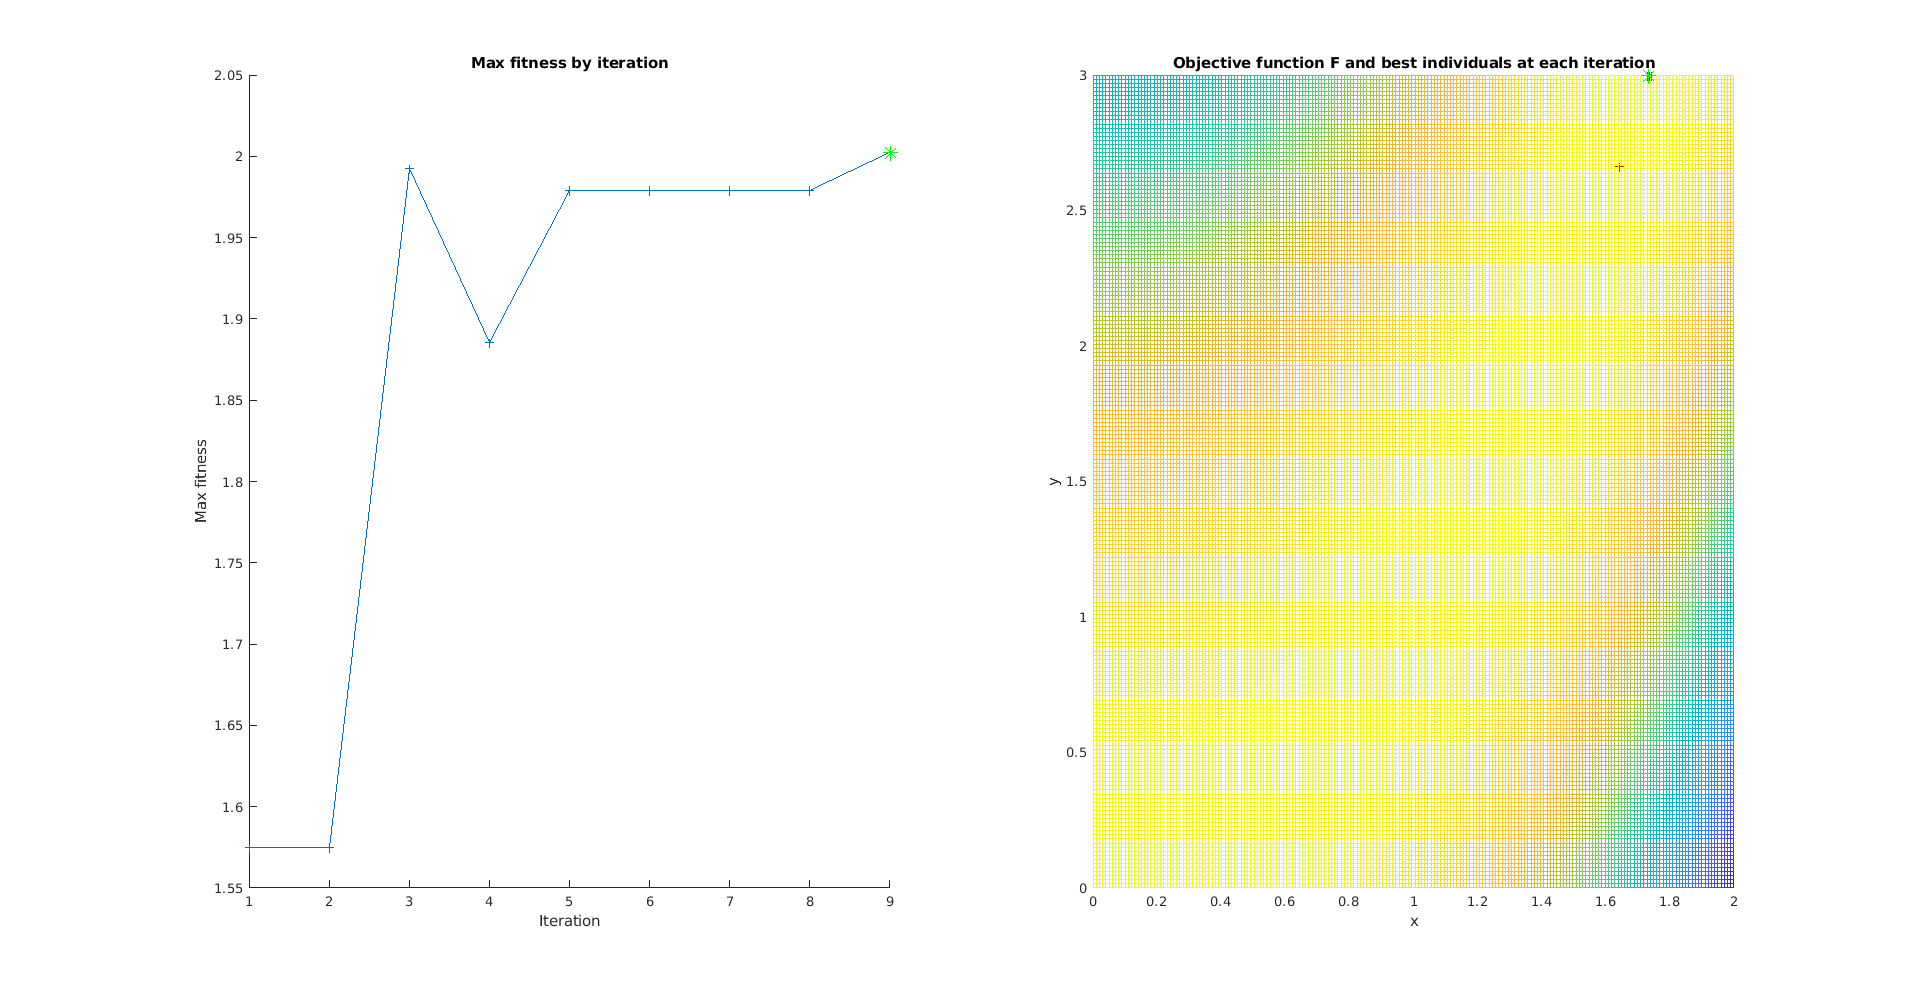
\includegraphics[width=\linewidth]{img/r_quick.png}
  \centering
  \captionsetup{justification=centering}
  \caption{Rosenbrock - $N = 100$, Unbiased tournament ($k = 4$), BLX-1, boundary mutation}
  \label{fig:r_quick}
\end{figure}

\begin{figure}
  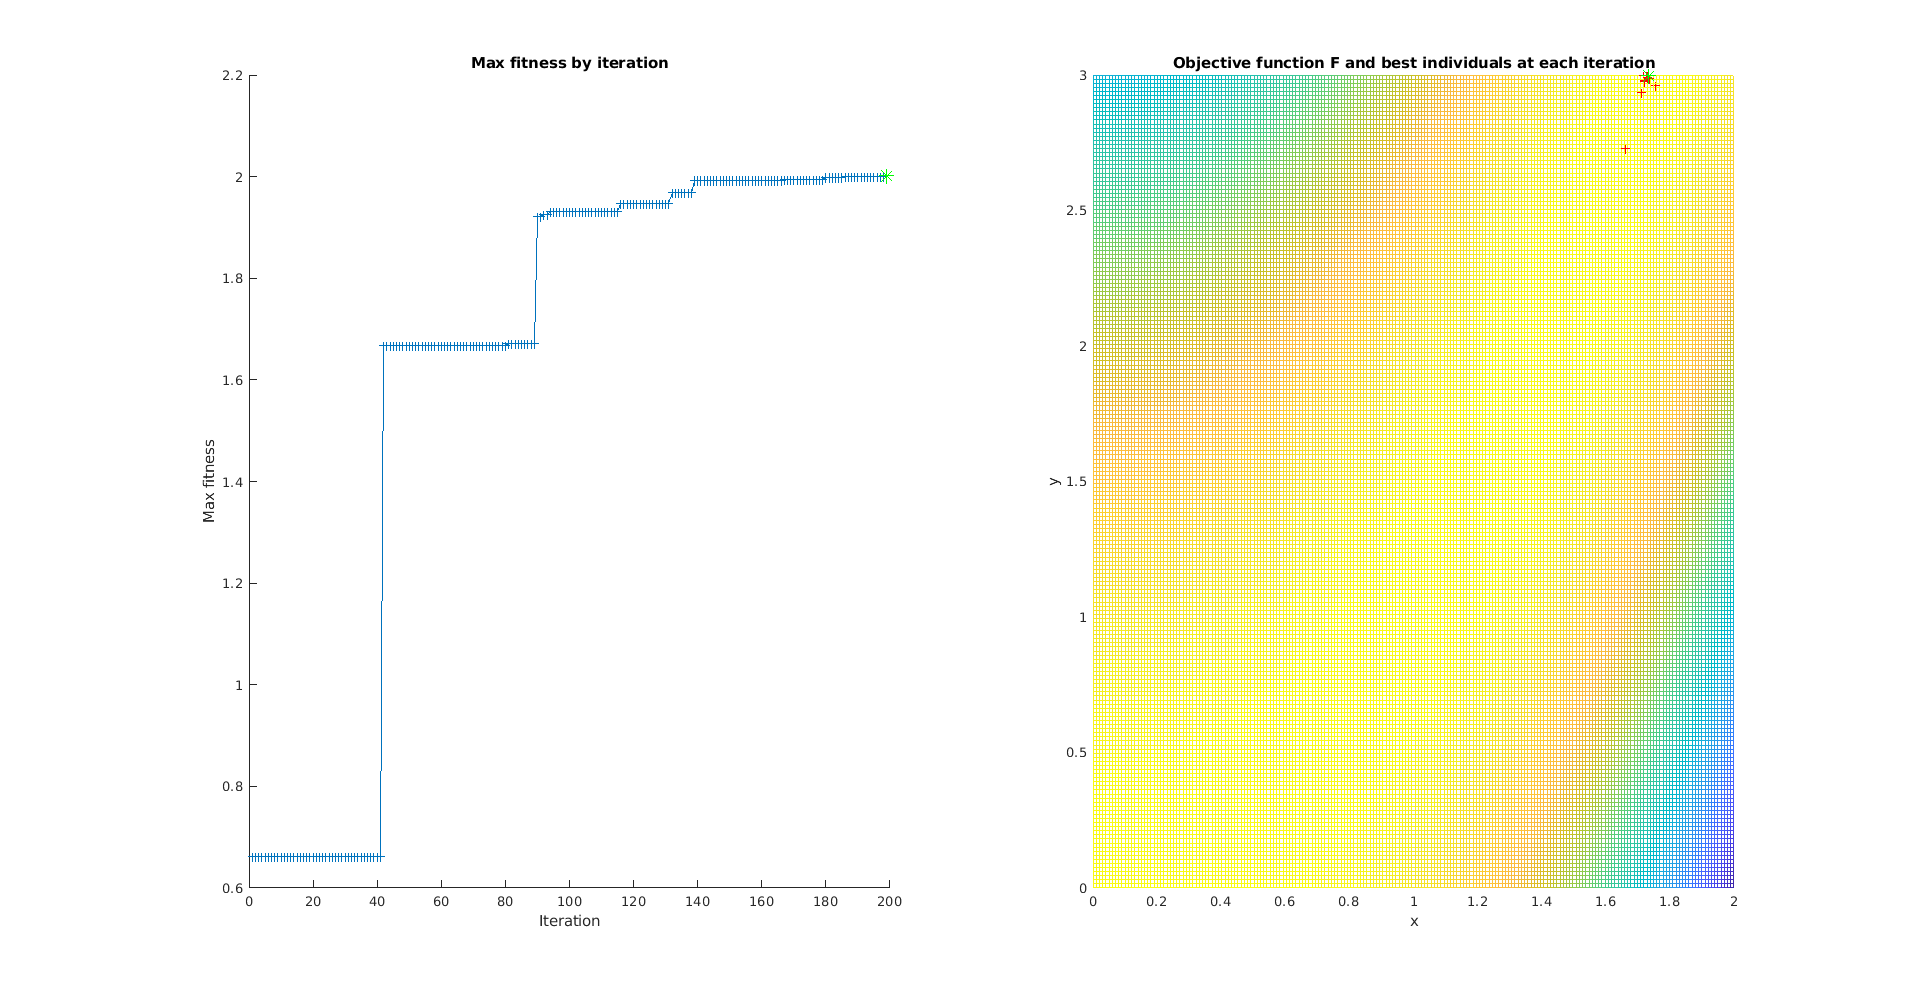
\includegraphics[width=\linewidth]{img/r_ss.png}
  \centering
  \captionsetup{justification=centering}
  \caption{Rosenbrock - $N = 10$, Steady State ($\lambda = 2$), BLX-1, non-linear ranking ($\alpha = 0.99$)}
  \label{fig:r_ss}
\end{figure}

\begin{figure}
  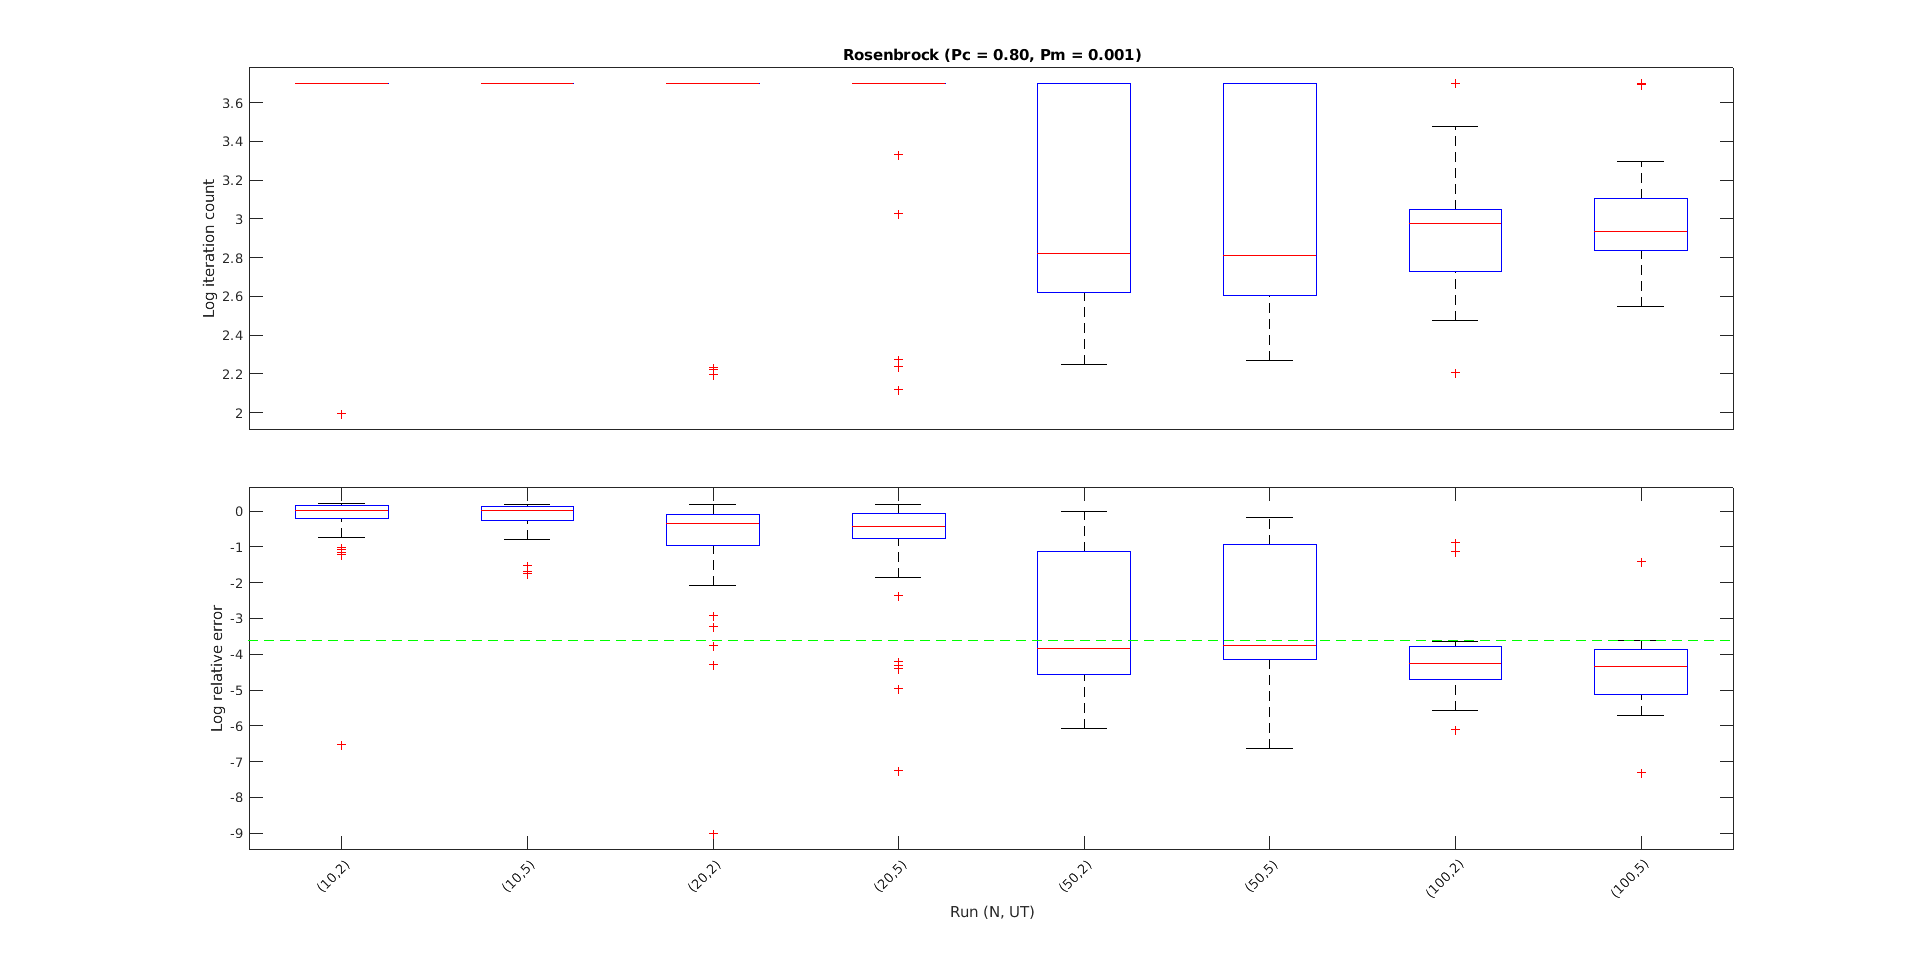
\includegraphics[width=\linewidth]{img/r_ss_test.png}
  \centering
  \captionsetup{justification=centering}
  \caption{Rosenbrock - Steady State ($\lambda = 2$), Unbiased tournament, BLX-1, non-linear ranking ($\alpha = 0.99$)}
  \label{fig:r_ss_test}
\end{figure}

%% Griewank
\begin{figure}
  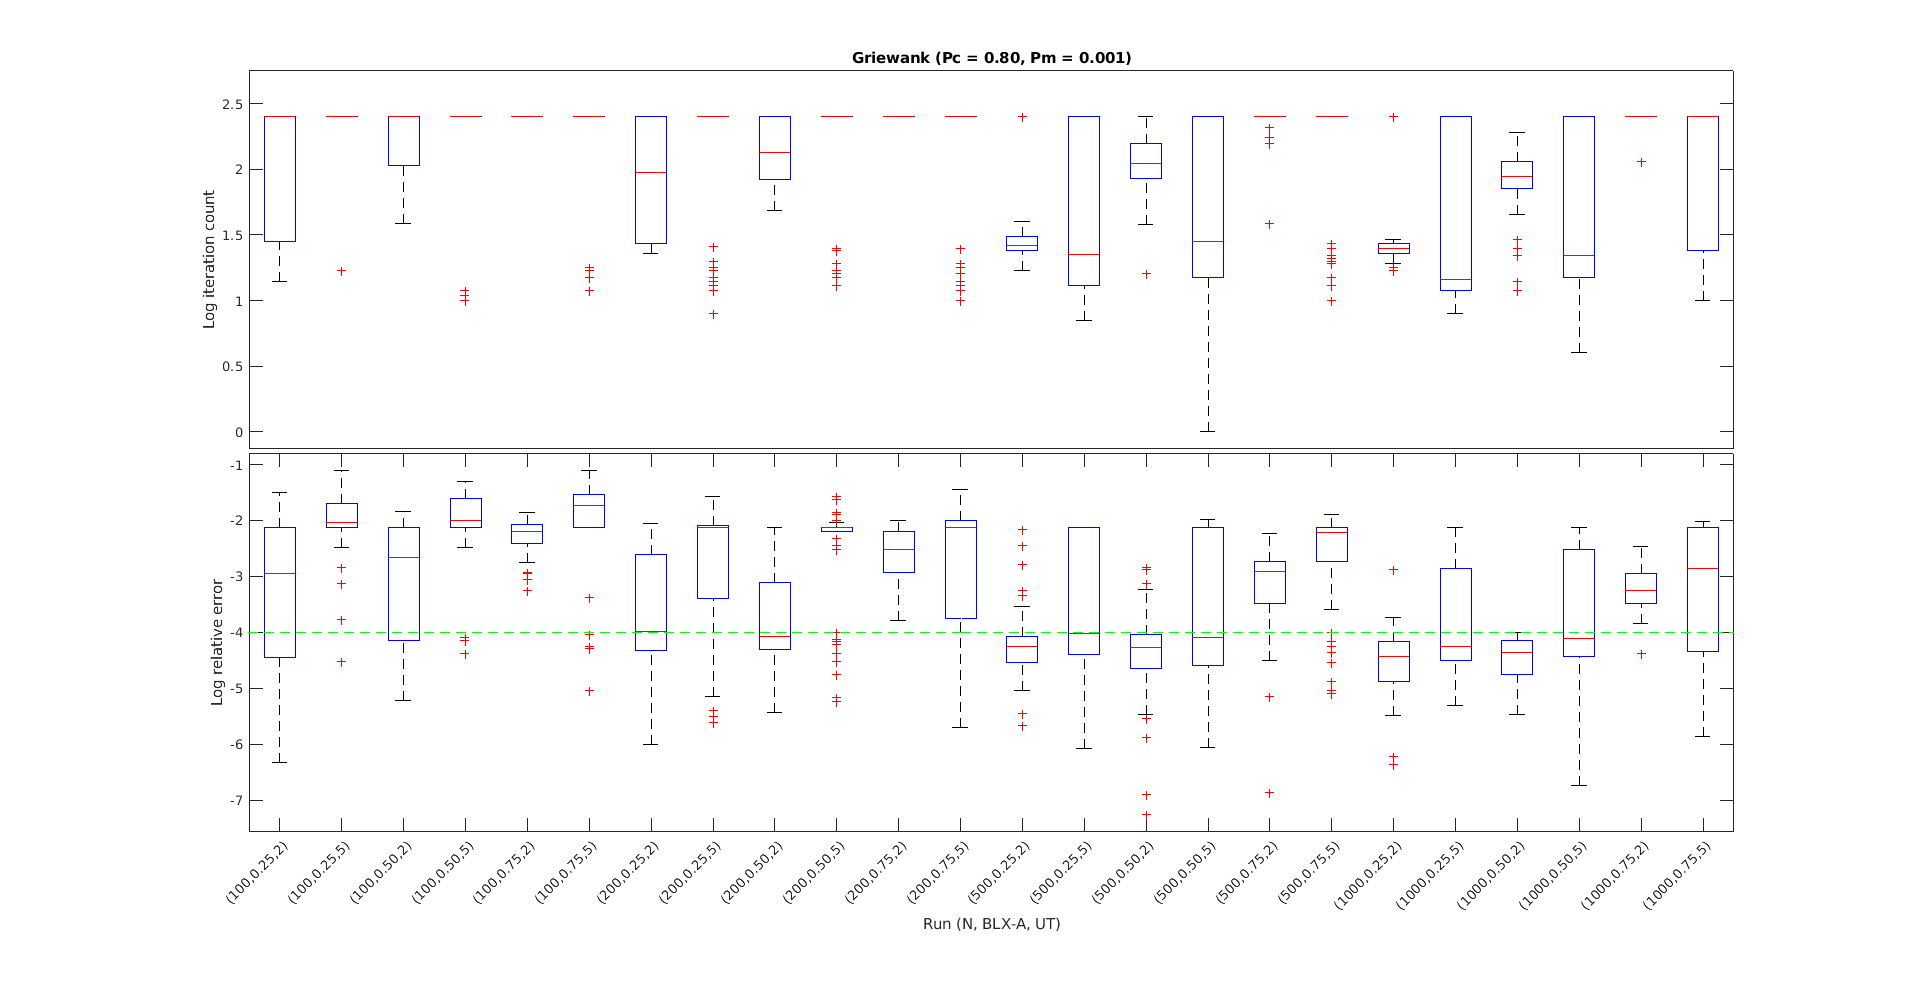
\includegraphics[width=\linewidth]{img/g_blx_ut_08_001.png}
  \centering
  \captionsetup{justification=centering}
  \caption{Griewank - BLX-$\alpha$, Unbiased tournament, $P_C = 0.8$, $P_M = 0.001$}
  \label{fig:g_blx_ut_08_001}
\end{figure}

\begin{figure}
  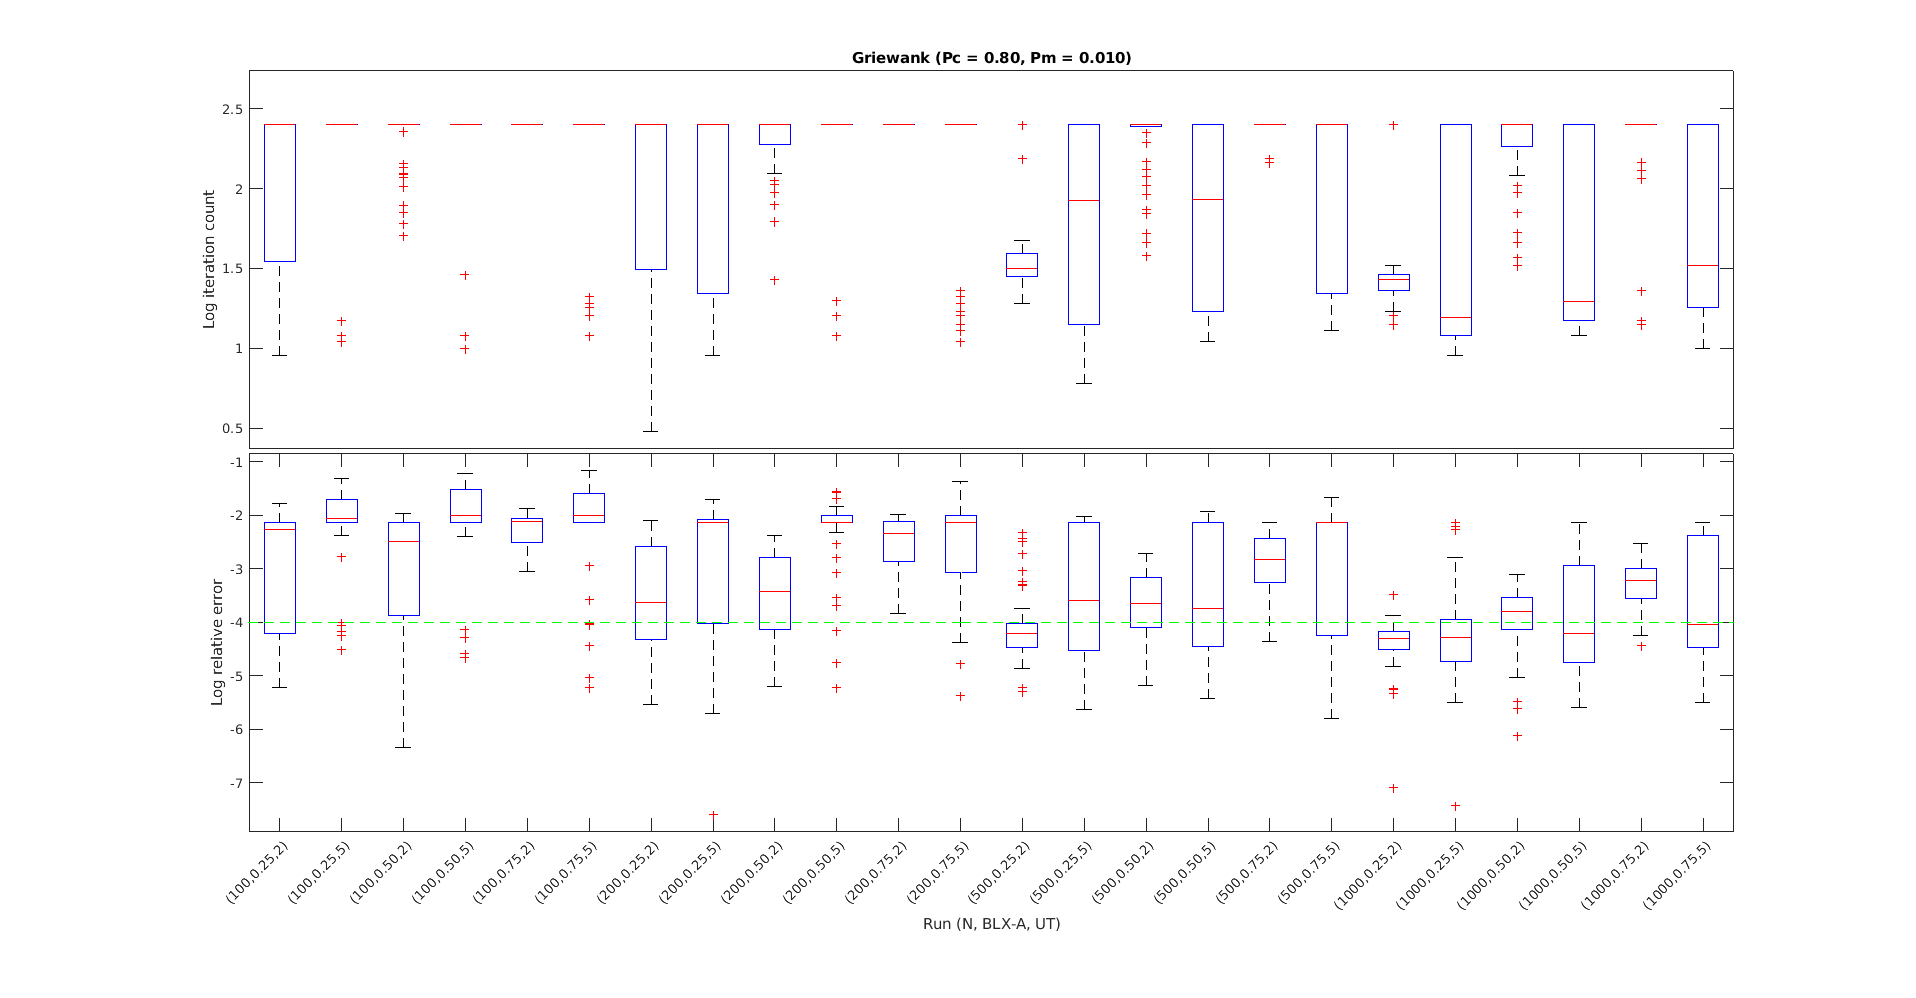
\includegraphics[width=\linewidth]{img/g_blx_ut_08_010.png}
  \centering
  \captionsetup{justification=centering}
  \caption{Griewank - BLX-$\alpha$, Unbiased tournament, $P_C = 0.8$, $P_M = 0.01$}
  \label{fig:g_blx_ut_08_010}
\end{figure}

\begin{figure}
  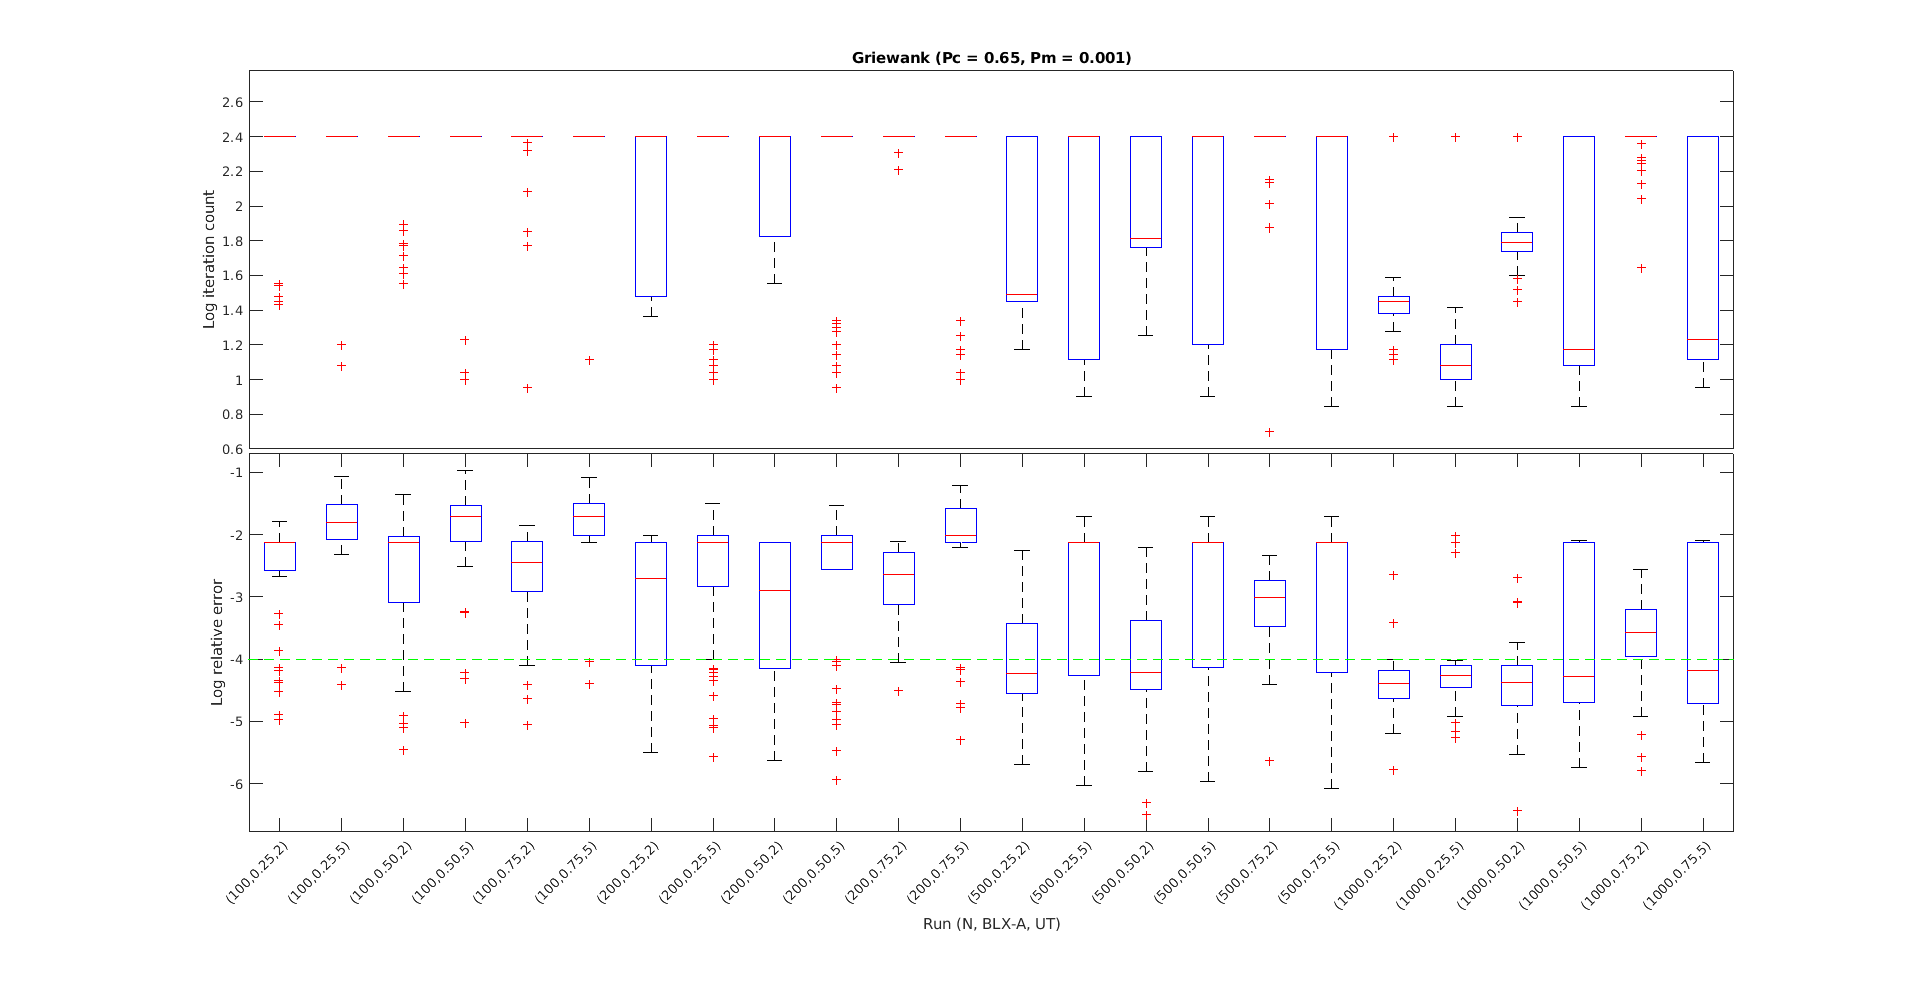
\includegraphics[width=\linewidth]{img/g_blx_ut_065_001.png}
  \centering
  \captionsetup{justification=centering}
  \caption{Griewank - BLX-$\alpha$, Unbiased tournament, $P_C = 0.65$, $P_M = 0.001$}
  \label{fig:g_blx_ut_065_001}
\end{figure}

\begin{figure}
  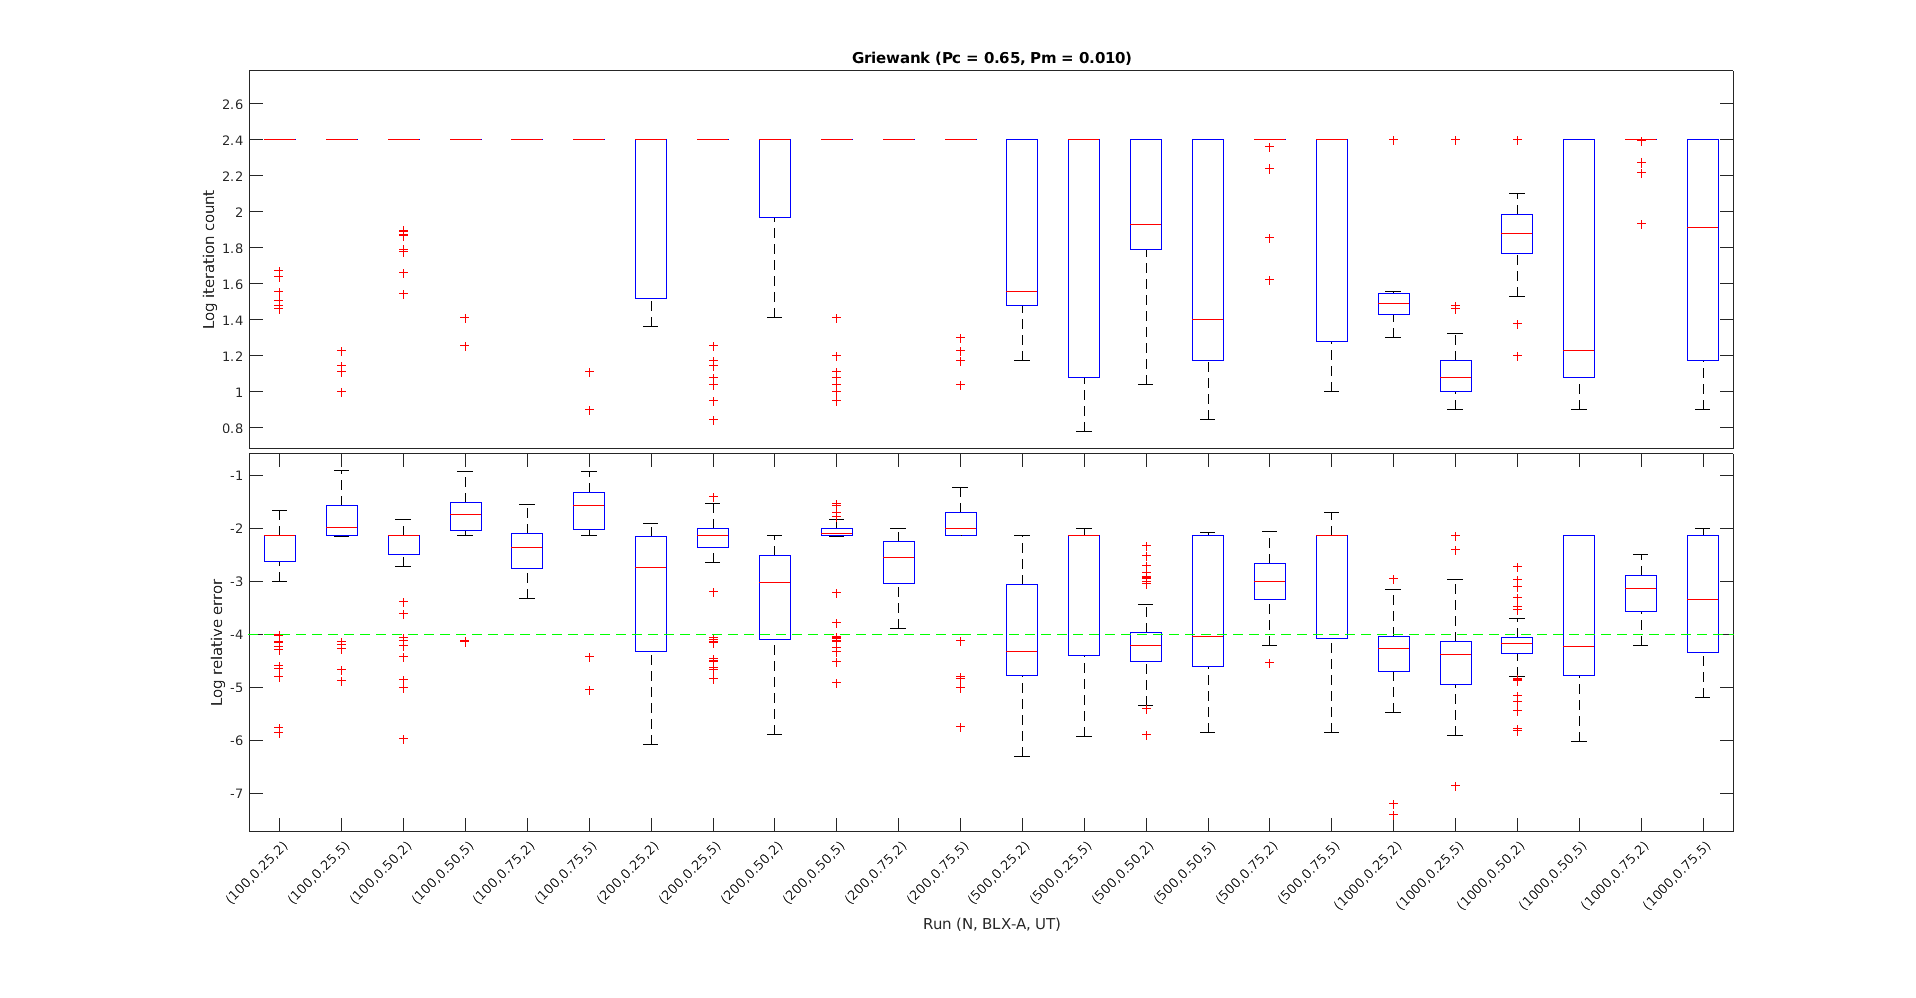
\includegraphics[width=\linewidth]{img/g_blx_ut_065_010.png}
  \centering
  \captionsetup{justification=centering}
  \caption{Griewank - BLX-$\alpha$, Unbiased tournament, $P_C = 0.65$, $P_M = 0.01$}
  \label{fig:g_blx_ut_065_010}
\end{figure}

\begin{figure}
  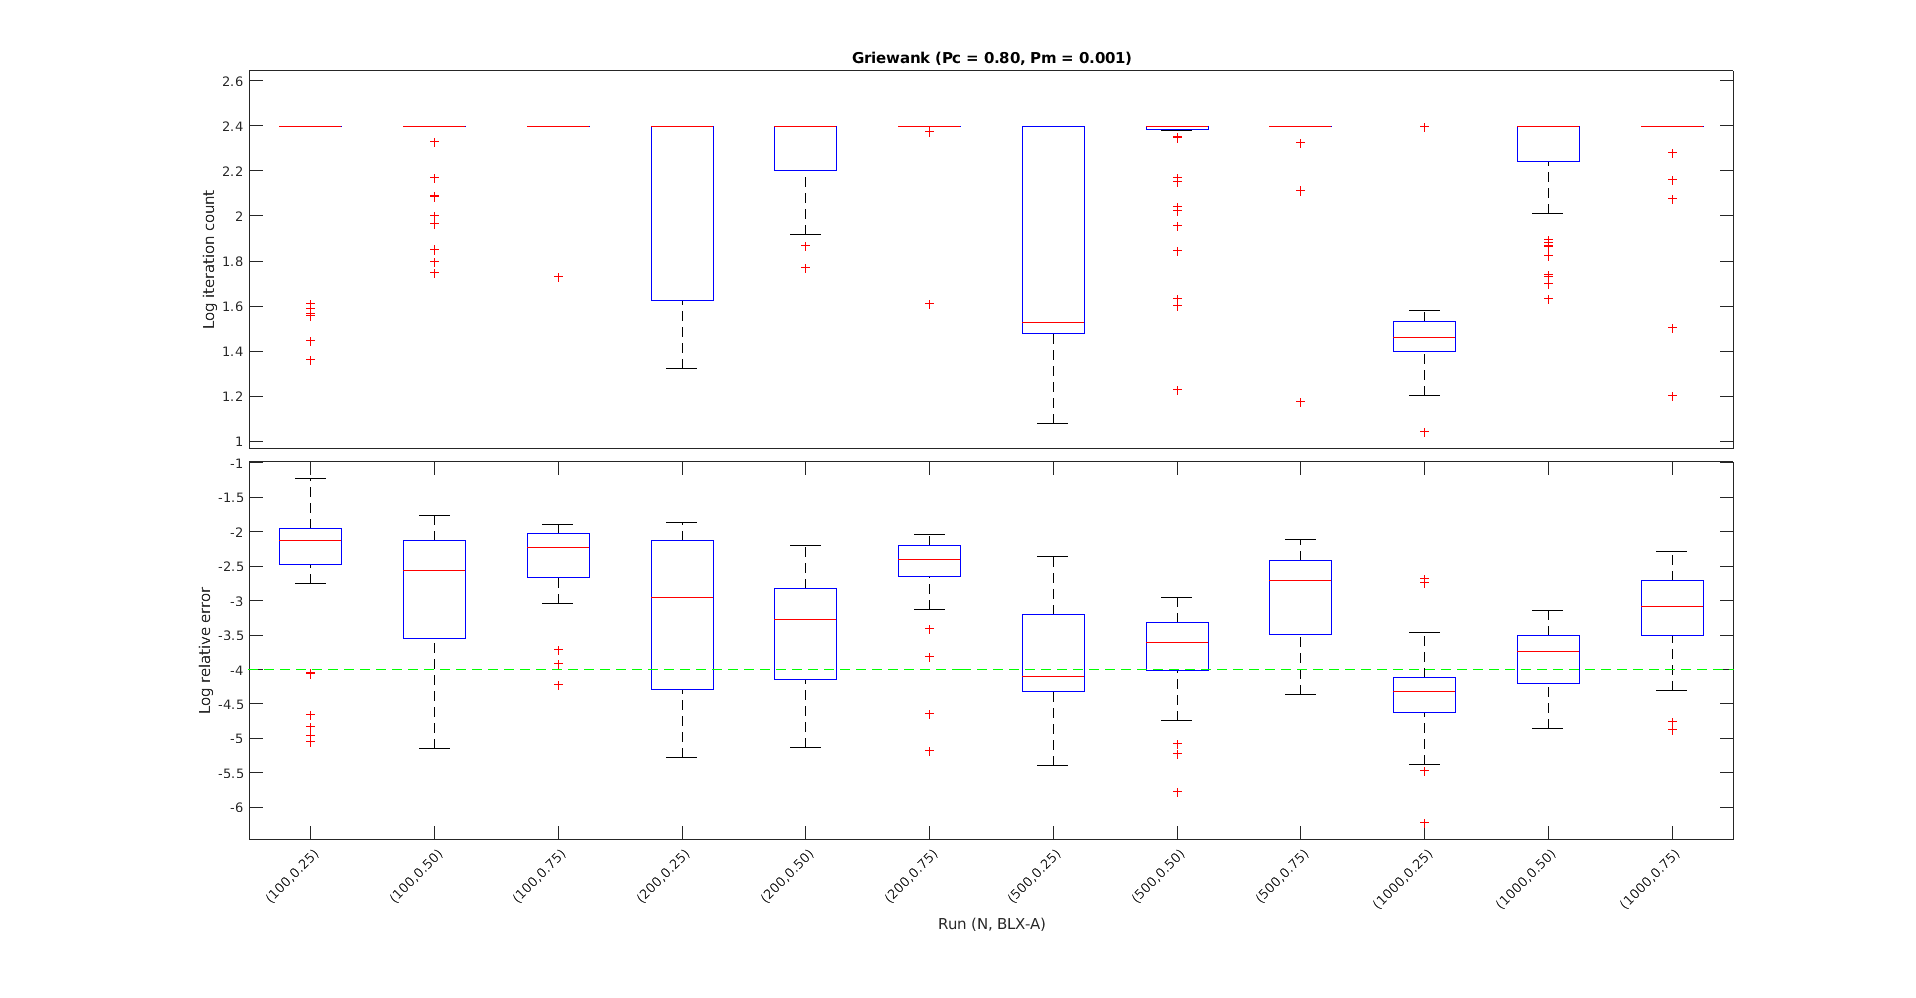
\includegraphics[width=\linewidth]{img/g_blx_w.png}
  \centering
  \captionsetup{justification=centering}
  \caption{Rosenbrock - BLX-$\alpha$, Wheel}
  \label{fig:g_blx_w}
\end{figure}

\begin{figure}
  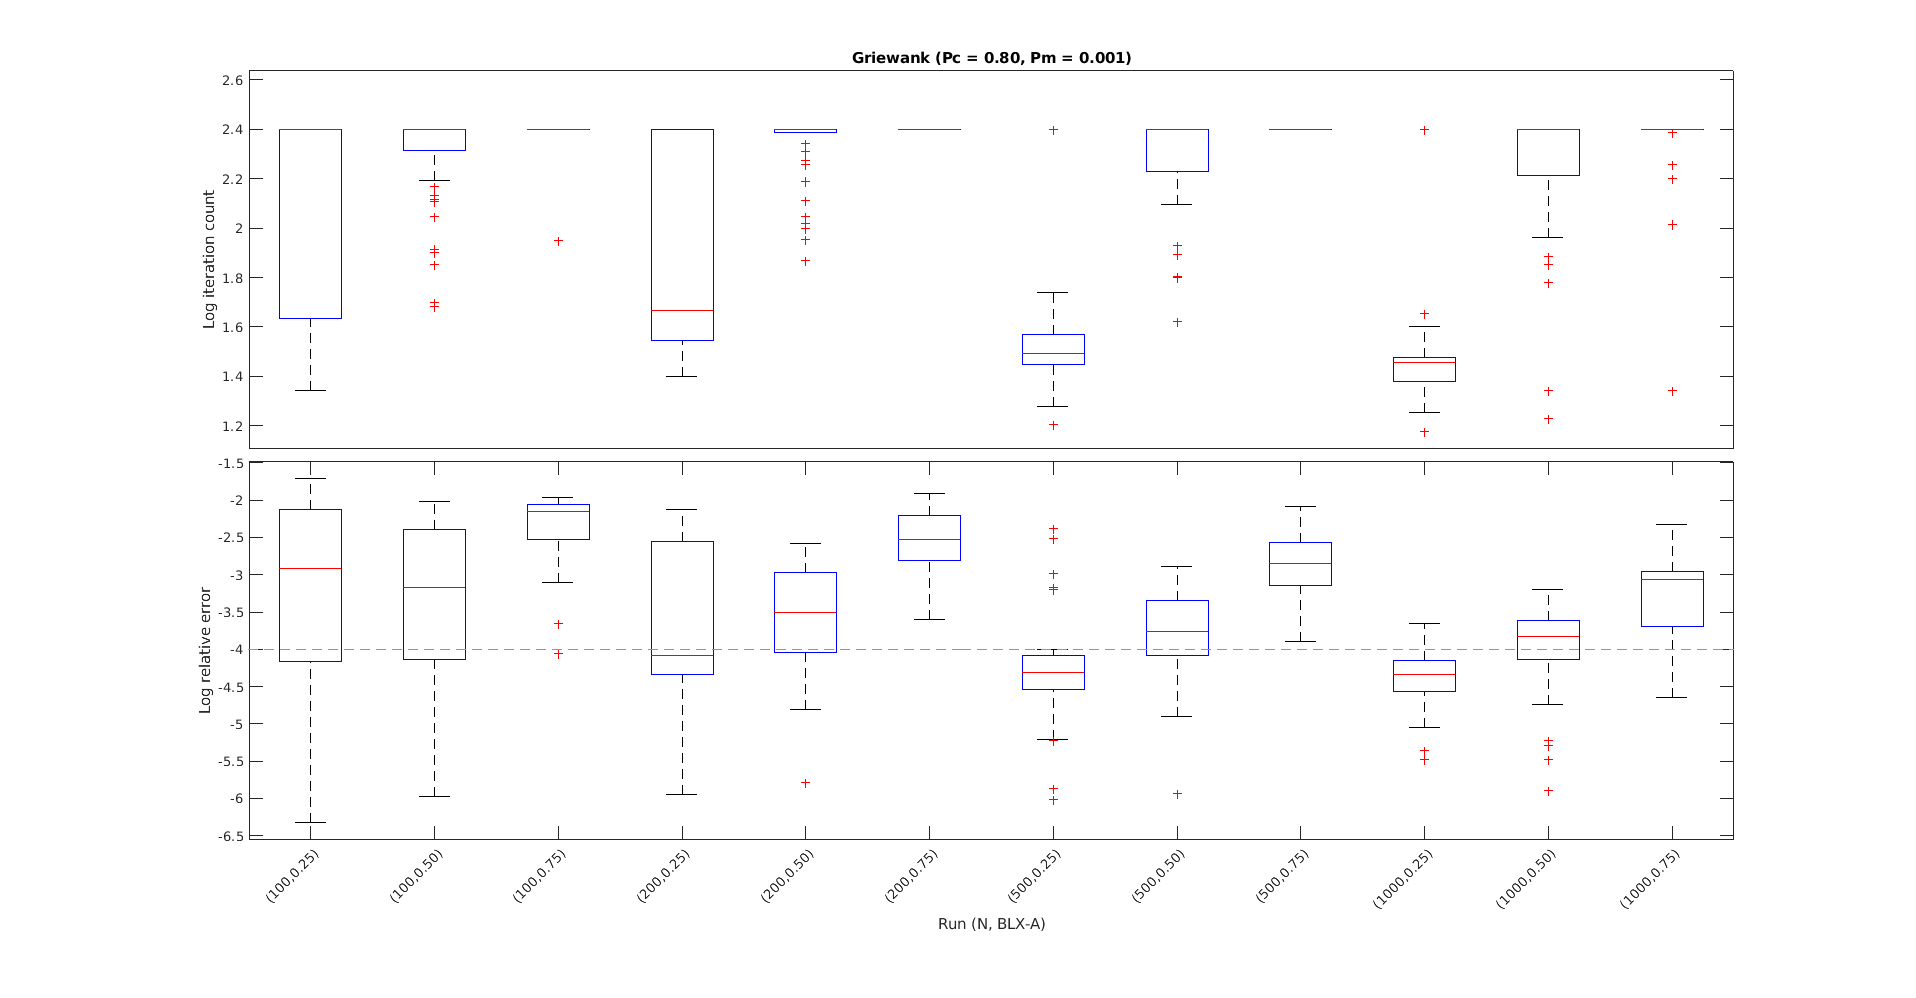
\includegraphics[width=\linewidth]{img/g_blx_sus.png}
  \centering
  \captionsetup{justification=centering}
  \caption{Rosenbrock - BLX-$\alpha$, Stochastic Universal Sampling}
  \label{fig:g_blx_sus}
\end{figure}

\begin{figure}
  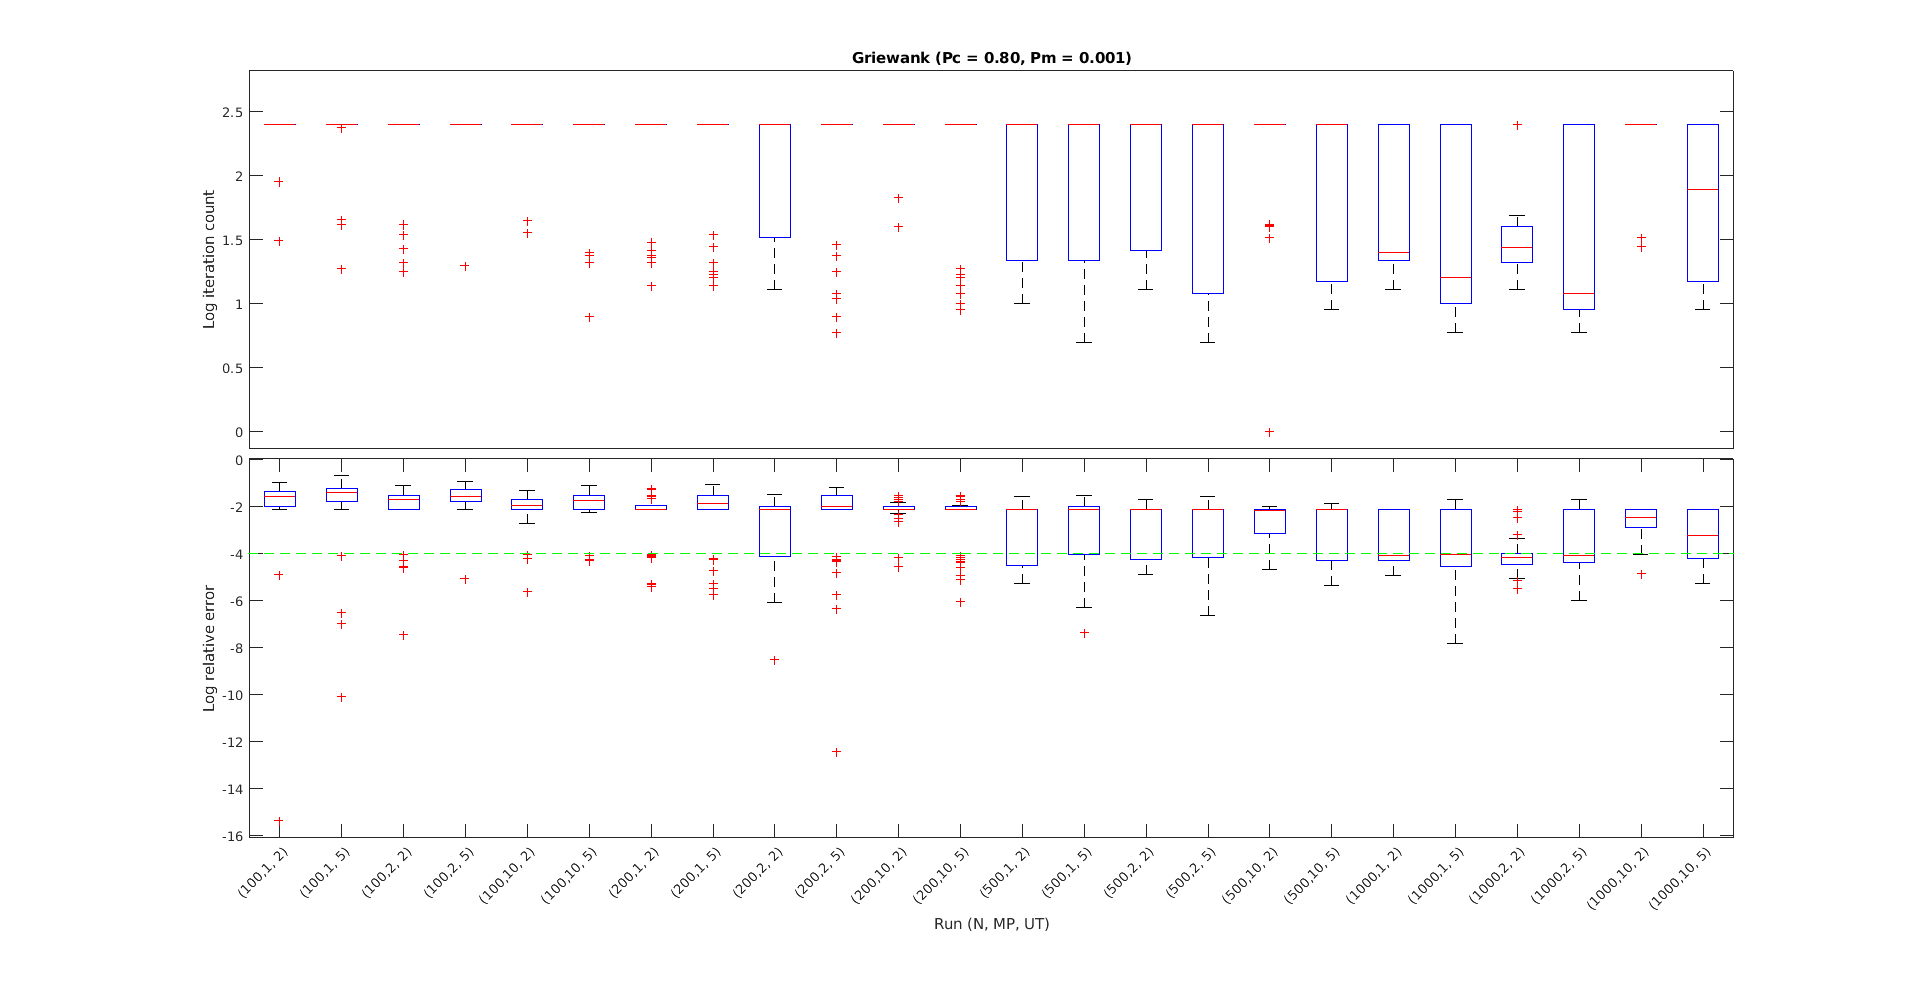
\includegraphics[width=\linewidth]{img/g_mp_ut.png}
  \centering
  \captionsetup{justification=centering}
  \caption{Griewank - Multi-point, Unbiased tournament}
  \label{fig:g_mp_ut}
\end{figure}

\begin{figure}
  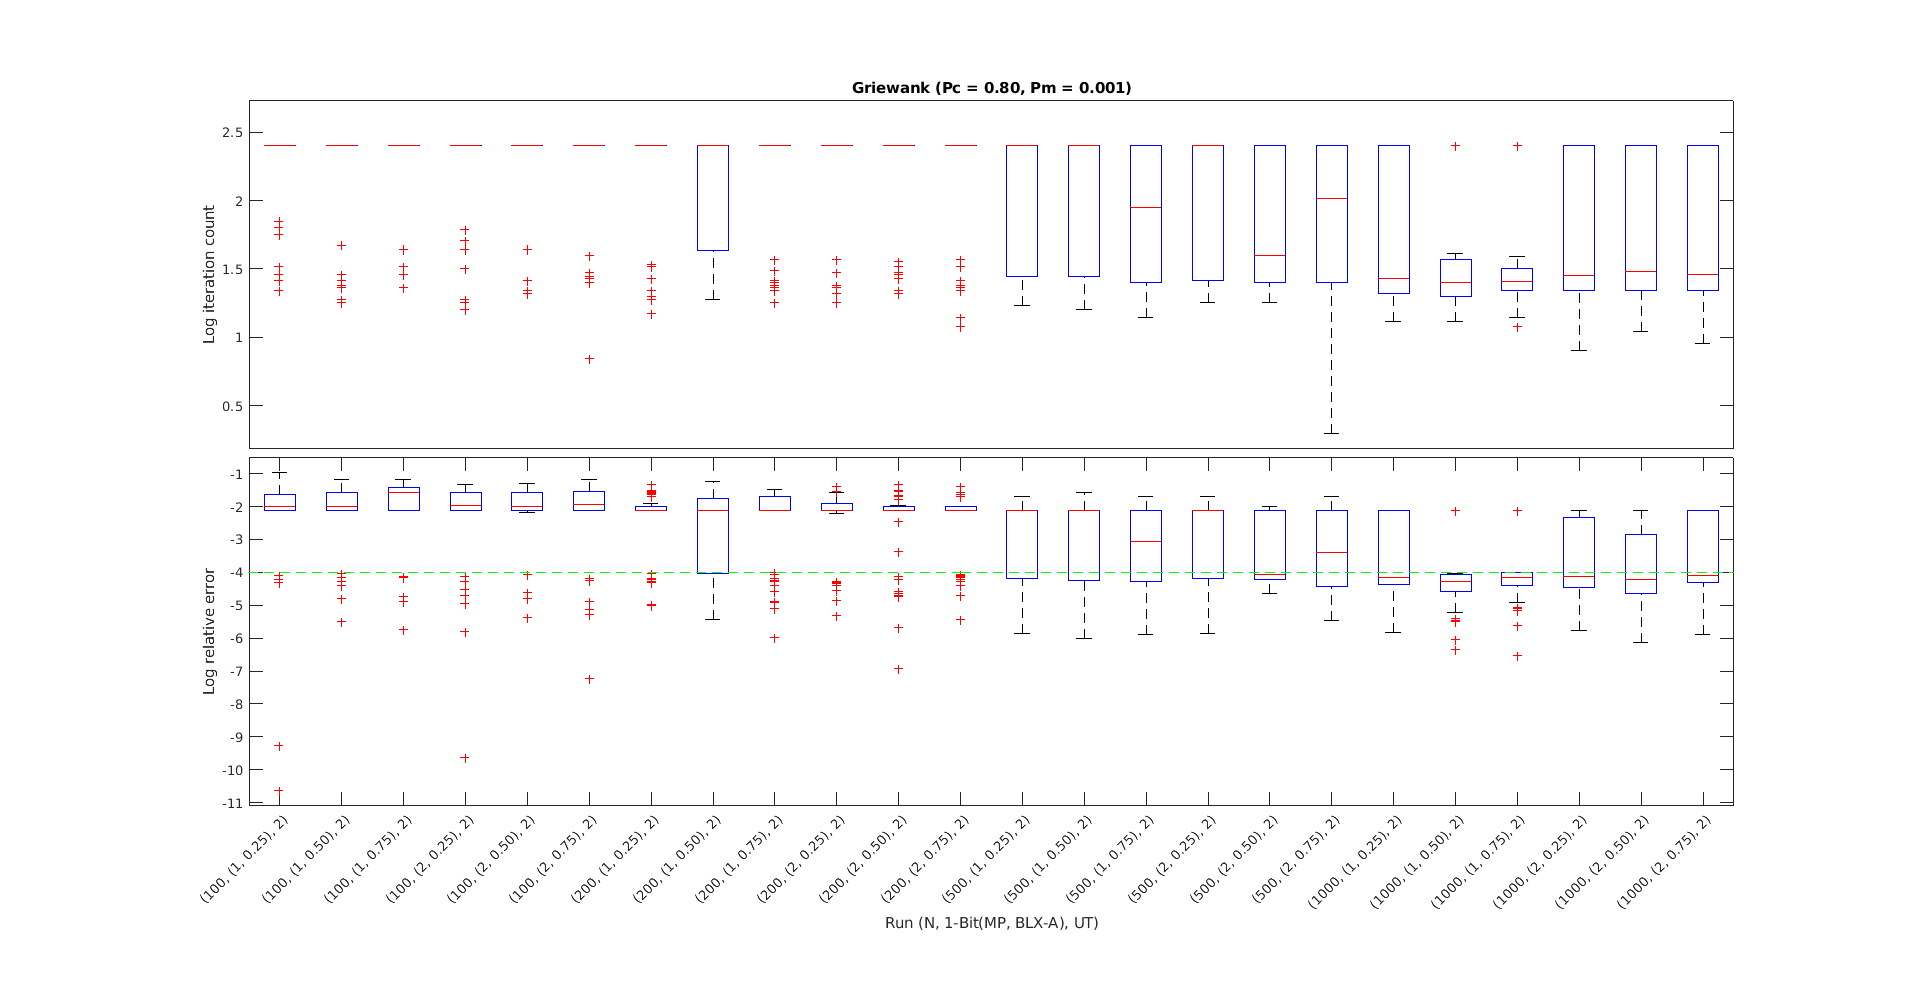
\includegraphics[width=\linewidth]{img/g_1b_ut.png}
  \centering
  \captionsetup{justification=centering}
  \caption{Griewank - 1-Bit Adaptation, Unbiased tournament}
  \label{fig:g_1b_ut}
\end{figure}
 
\begin{figure}
  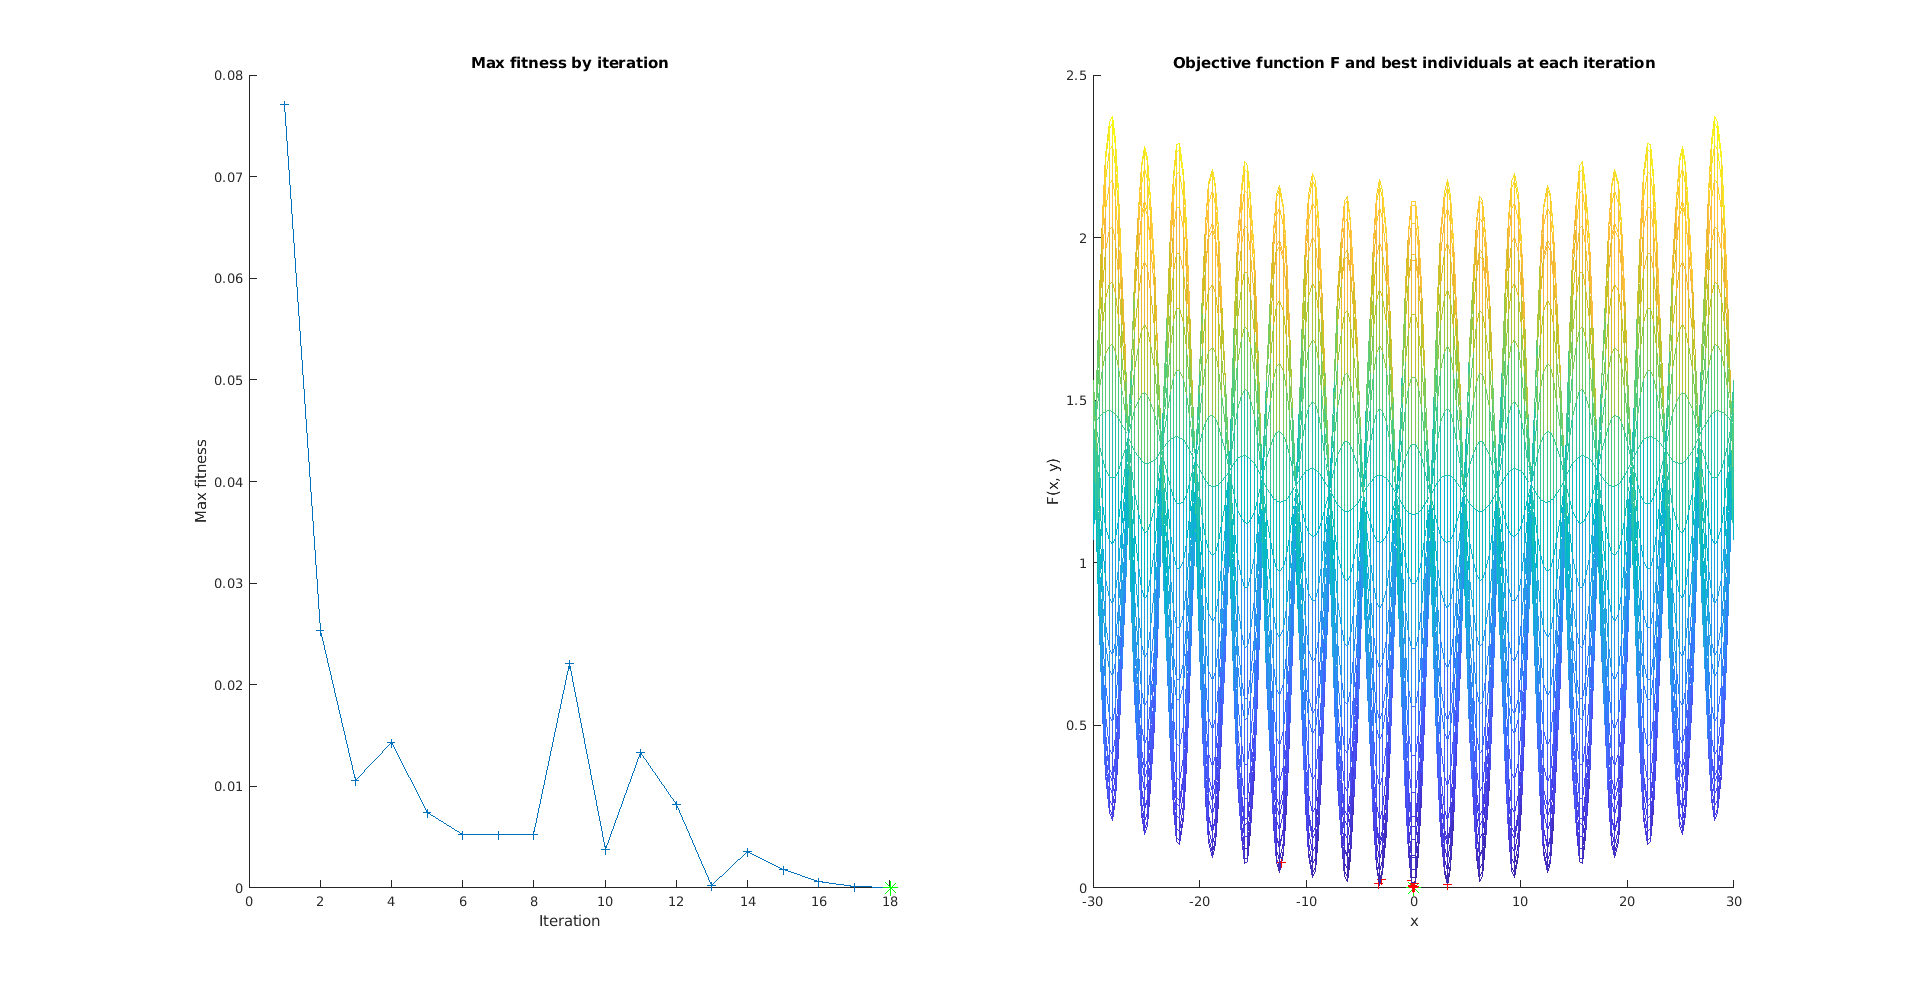
\includegraphics[width=\linewidth]{img/g_quick.png}
  \centering
  \captionsetup{justification=centering}
  \caption{Griewank - $N = 500$, Unbiased tournament ($k = 2$), BLX-0, Non-uniform mutation ($b = 2$), non-linear ranking ($\alpha = 0.99$)}
  \label{fig:g_quick}
\end{figure}

\begin{figure}
  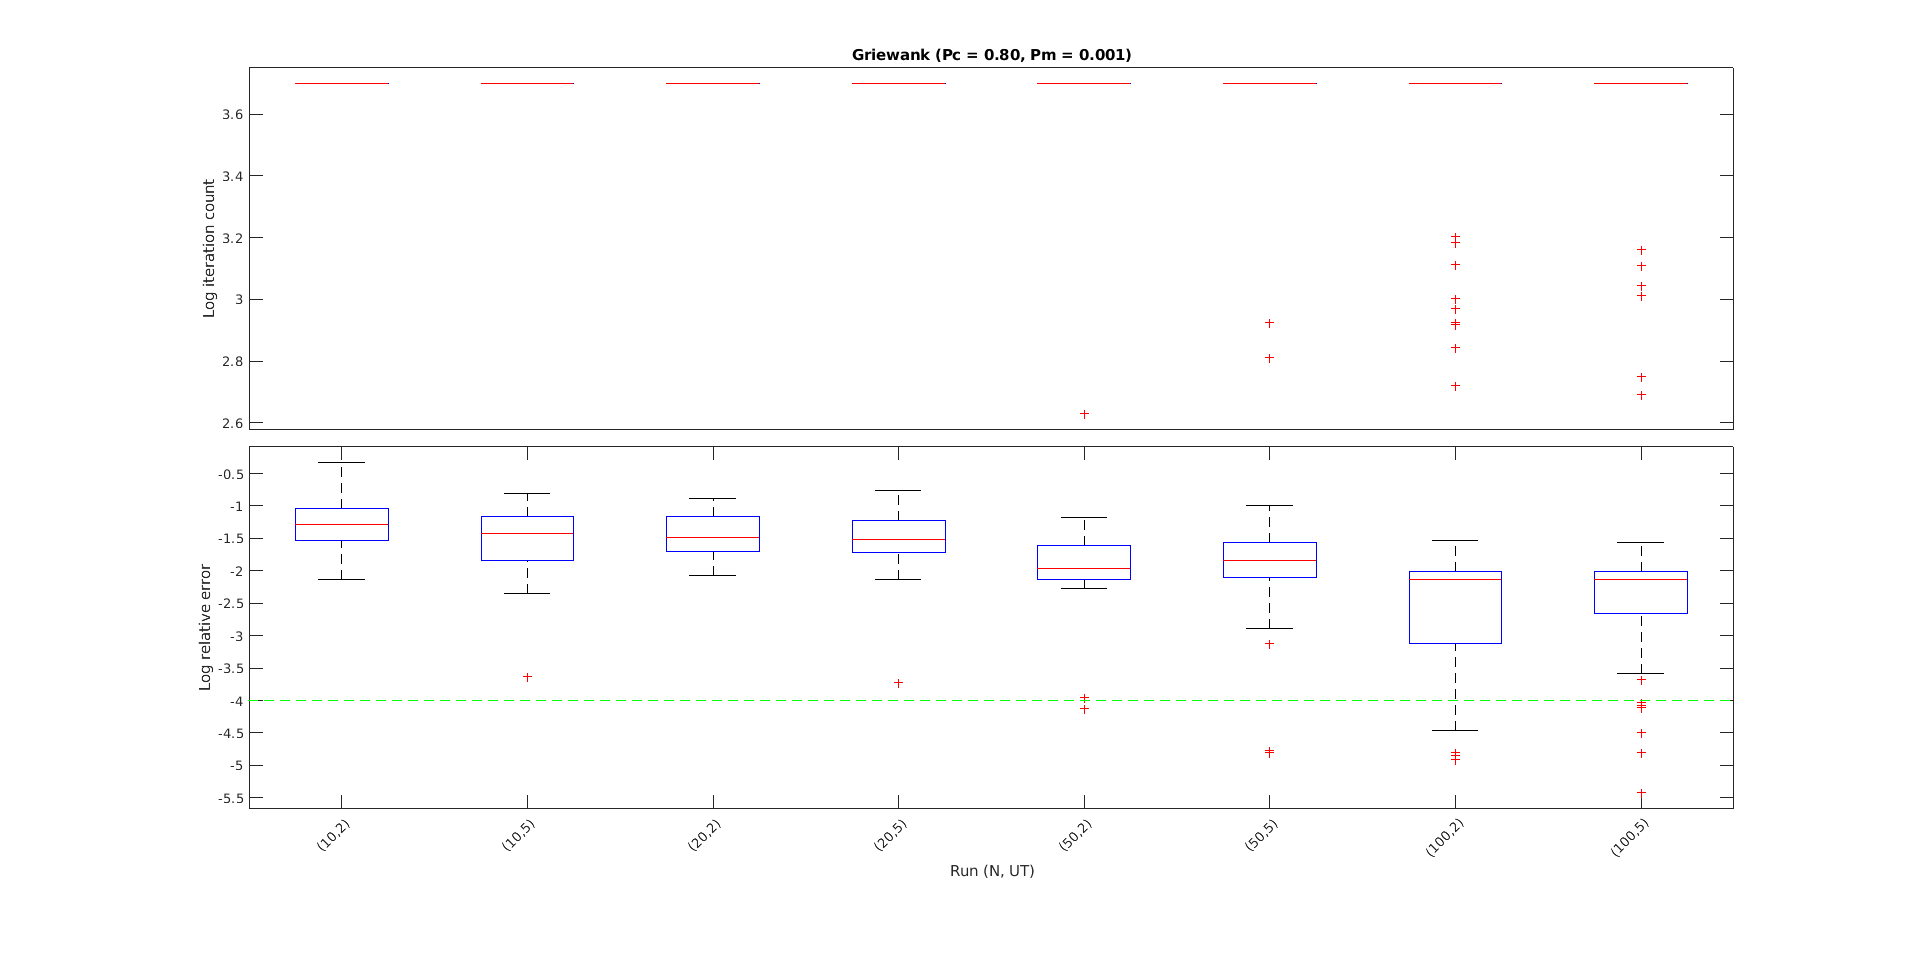
\includegraphics[width=\linewidth]{img/g_ss_test.png}
  \centering
  \captionsetup{justification=centering}
  \caption{Griewank - Steady State ($\lambda = 2$), Unbiased tournament, BLX-0, non-linear ranking ($\alpha = 0.99$)}
  \label{fig:g_ss_test}
\end{figure}

\end{document}

%%% Local Variables:
%%% mode: latex
%%% TeX-master: t
%%% End:
